\documentclass[12pt, a4paper]{article}

% ----- Packages -----
\usepackage[utf8]{inputenc}
\usepackage[T1]{fontenc}
\usepackage[french]{babel}
\usepackage{geometry}
\geometry{margin=2.5cm, headheight=14pt}
\usepackage{graphicx}
\usepackage{float}
\usepackage{hyperref}
\usepackage{xcolor}
\usepackage{enumitem}
\usepackage{setspace}
\usepackage{titlesec}
\usepackage{fancyhdr}
\usepackage{booktabs}
\usepackage{amsmath}
\usepackage{amssymb}
\usepackage{parskip}
\usepackage{caption}
\usepackage{natbib}

% ----- Configuration -----
\hypersetup{
    colorlinks=true,
    linkcolor=blue!60!black,
    citecolor=blue!60!black,
    urlcolor=blue!60!black
}

\onehalfspacing

\pagestyle{fancy}
\fancyhf{}
\fancyhead[L]{\small\leftmark}
\fancyhead[R]{\small\thepage}
\fancyfoot[C]{}
\renewcommand{\headrulewidth}{0.4pt}

\titleformat{\section}{\Large\bfseries}{\thesection.}{0.5em}{}
\titleformat{\subsection}{\large\bfseries}{\thesubsection.}{0.5em}{}
\titleformat{\subsubsection}{\normalsize\bfseries}{\thesubsubsection.}{0.5em}{}

% Encadrés titrés (bandeau de titre + fond coloré)
\newsavebox{\encadrebox}
\newenvironment{encadre}[1]{%
  \par\bigskip
  \def\encadretitre{#1}%
  \begin{lrbox}{\encadrebox}%
  \begin{minipage}{\dimexpr\linewidth-2\fboxsep-2\fboxrule\relax}%
  \setlength{\parskip}{6pt}%
}{%
  \end{minipage}%
  \end{lrbox}%
  \noindent
  \fcolorbox{blue!50!black}{blue!50!black}{%
    \begin{minipage}{\dimexpr\linewidth-2\fboxsep-2\fboxrule\relax}%
    \textcolor{white}{\textbf{\encadretitre}}%
    \end{minipage}}\par\nointerlineskip
  \noindent
  \fcolorbox{blue!50!black}{blue!5!white}{\usebox{\encadrebox}}%
  \par\bigskip
}

% Chemin des images
\graphicspath{{output/plots_WD/}{output/plots/}{./}}

% ----- Début du document -----
\begin{document}

% ========================================
% PAGE DE TITRE
% ========================================
\begin{titlepage}
\centering
\vspace*{1cm}

{\LARGE\bfseries Effets macroéconomiques de la transition bas carbone\\
dans les pays en développement :\\
une analyse comparative Tunisie--Mexique\\
à l'aide du modèle ThreeME\par}

\vspace{1.5cm}

{\large Sami Mena\textsuperscript{a}, Victor Scache\textsuperscript{a}, Louis Viard\textsuperscript{a}, Meriem Hamdi-Cherif\textsuperscript{b,}\footnote{Corresponding author: \href{mailto:meriem.hamdicherif@sciencespo.fr}{meriem.hamdicherif@sciencespo.fr}}\par}

\vspace{0.8cm}

{\normalsize \textsuperscript{a} M2 EEET, Parcours Modélisation Prospective, Université Paris-Saclay\\
\textsuperscript{b} OFCE -- Observatoire français des conjonctures économiques, SciencesPo\par}

\vspace{1.5cm}

\textbf{Résumé.} Cet article propose une évaluation quantitative des effets macroéconomiques et environnementaux de stratégies nationales bas carbone (SNBC) dans deux économies en développement aux profils énergétiques divergents : la Tunisie, importatrice nette d'hydrocarbures, et le Mexique, exportateur net. À l'aide du modèle d'équilibre général calculable néo-keynésien ThreeME, nous simulons des scénarios de transition énergétique ambitieux à l'horizon 2050, combinant taxation carbone, suppression des subventions fossiles et déploiement des énergies renouvelables, avec recyclage intégral des recettes fiscales. Les résultats montrent que ces instruments, lorsqu'ils sont combinés, permettent de réduire les émissions de 60 à 69\,\% en 2050 tout en générant un double dividende économique. Toutefois, une asymétrie structurelle apparaît : la Tunisie bénéficie d'un effet de relance immédiat par la réduction de la facture énergétique extérieure et l'investissement vert, tandis que le Mexique doit gérer un choc d'offre négatif sur son secteur extractif, générant une réallocation sectorielle plus complexe. À notre connaissance, cette étude est la première à proposer une comparaison systématique, à l'aide d'un modèle d'équilibre général calculable, des impacts macroéconomiques de la transition entre un pays en développement exportateur et un pays en développement importateur de combustibles fossiles.

\vspace{0.8cm}

\textbf{Mots-clés :} Transition bas carbone, Taxe carbone, Modèle d'équilibre général calculable (MEGC), Double dividende, Pays en développement, Tunisie, Mexique.

\textbf{Classification JEL :} Q48, Q52, Q58, O55, C68

\vfill
\end{titlepage}

% ========================================
% TABLE DES MATIÈRES
% ========================================
\newpage
\tableofcontents
\newpage

% ========================================
% ENCADRÉ HIGHLIGHTS
% ========================================
\begin{encadre}{Highlights}
\begin{itemize}[leftmargin=*]
    \item Première évaluation comparative par MEGC néo-keynésien de la transition bas carbone entre un pays en développement importateur (Tunisie) et exportateur (Mexique) d'énergie fossile.
    \item Le recyclage intégral des recettes de la taxe carbone est une condition nécessaire à l'obtention d'un double dividende économique.
    \item La transition représente un choc asymétrique : opportunité de souveraineté énergétique pour l'importateur, défi de restructuration industrielle pour l'exportateur.
    \item L'investissement vert et les créations d'emplois dans les secteurs bas carbone compensent largement les pertes dans les secteurs fossiles, mais nécessitent un accompagnement des réallocations sectorielles.
\end{itemize}
\end{encadre}

\vspace{1cm}

% ========================================
% RECOMMANDATIONS
% ========================================
\begin{encadre}{Recommandations de politiques publiques}

\textbf{Associer la tarification carbone à un recyclage visible et ciblé.} Le recyclage des recettes est essentiel pour éviter un effet récessif et renforcer l'acceptabilité sociale. Les fonds issus de la taxe carbone devraient financer des transferts vers les ménages, en particulier les plus vulnérables, ainsi qu'un allègement ciblé des coûts du travail ou de la production.

\textbf{Adapter le scénario à la structure énergétique du pays.} Pour les pays importateurs nets d'énergie, la transition peut réduire la dépendance extérieure et améliorer la balance commerciale : les politiques doivent accélérer le développement des énergies renouvelables domestiques. Pour les pays exportateurs d'hydrocarbures, la transition implique une transformation productive plus profonde, qui doit s'accompagner d'une stratégie de diversification industrielle.

\textbf{Accompagner les réallocations sur le marché du travail.} Même en cas de gains d'emplois agrégés, des pertes sectorielles localisées sont inévitables. Des politiques de formation, de reconversion et de mobilité professionnelle sont nécessaires pour limiter les coûts sociaux et maintenir le soutien politique à la transition.
\end{encadre}

\newpage

% ========================================
% 1. INTRODUCTION
% ========================================
\section{Introduction}
\label{sec:introduction}

\subsection{Contexte international et hétérogénéité du Sud}

L'Accord de Paris, adopté en 2015 dans le cadre de la Convention-Cadre des Nations Unies sur les Changements Climatiques (CCNUCC), appelle les États signataires à mettre en \oe{}uvre des politiques climatiques ambitieuses afin d'atteindre la neutralité carbone au cours de la seconde moitié du XXI\textsuperscript{e} siècle. Pour limiter le réchauffement global à un niveau inférieur à 2\,$^{\circ}$C par rapport à l'ère préindustrielle, un équilibre entre les émissions de gaz à effet de serre (GES) et leur absorption devra être atteint (UNFCCC, 2015). Dans un rapport spécial publié en octobre 2018, le Groupe d'experts intergouvernemental sur l'évolution du climat (GIEC) a mis en évidence que limiter le réchauffement à 1,5\,$^{\circ}$C --- plutôt que 2\,$^{\circ}$C --- permettrait d'éviter les conséquences les plus graves du changement climatique. Pour atteindre cet objectif, une réduction des émissions mondiales de 45\,\% d'ici 2030 par rapport aux niveaux de 2010 est indispensable, ainsi qu'une neutralité carbone globale à l'horizon 2050 (GIEC, 2018).

Conformément à l'article 4 de l'Accord, les gouvernements sont incités à activer deux leviers complémentaires : d'une part, les contributions déterminées au niveau national (CDN), qui définissent les engagements climatiques de chaque pays à moyen terme ; d'autre part, la stratégie nationale bas carbone (SNBC), qui vise à instaurer une trajectoire climatique cohérente à long terme en couvrant l'ensemble des secteurs économiques. Ces stratégies visent une décarbonation profonde à l'horizon 2050, en alignant les politiques nationales sur les objectifs mondiaux de réduction des GES.

Face à cette urgence climatique, les gouvernements sont appelés à mener des réformes structurelles de grande ampleur. Le secteur énergétique, en tant que principal émetteur de GES à l'échelle mondiale, occupe une place centrale dans cette transformation. Réformer rapidement et profondément les systèmes énergétiques apparaît comme un levier essentiel pour orienter les trajectoires nationales vers la neutralité carbone (IEA, 2021 ; IPCC, 2022 ; Sovacool et al., 2015).

Cependant, si les effets macroéconomiques de ces stratégies sont souvent étudiés pour les pays les plus développés économiquement --- notamment la France (Callonnec et al., 2025 ; Hamdi-Cherif et al., 2025), l'Allemagne (Böhringer et al., 2021 ; Lutz et al., 2021), l'Espagne (Böhringer et al., 2019) ou l'Union européenne dans son ensemble (Fragkos et al., 2021 ; Landis et al., 2021) ---, les analyses macroéconomiques des transitions bas carbone dans les pays en développement restent beaucoup plus rares (Lepault et Lecocq, 2021).

Or, dans l'histoire des négociations climatiques et des différentes COP, un antagonisme persistant oppose les pays du Nord et ceux du Sud. Le \textit{Global South} s'est longtemps présenté comme porteur d'une voix unique face aux pays industrialisés. Pourtant, si l'on ouvre cette <<~boîte~>> du Sud, on y trouve des réalités sensiblement différentes : les petits États insulaires vulnérables menacés de disparition, les grands émergents disposant d'une puissance économique considérable, mais aussi des pays intermédiaires aux trajectoires de développement très diverses. En matière de transition énergétique, ces spécificités nationales conditionnent fondamentalement la nature et l'ampleur des impacts macroéconomiques. Un pays en développement importateur net d'énergie fossile n'est pas confronté aux mêmes enjeux qu'un pays exportateur : pour le premier, la transition peut représenter une opportunité de souveraineté énergétique et de réduction de la facture extérieure ; pour le second, elle implique un processus de restructuration industrielle potentiellement coûteux à moyen terme.

C'est précisément cette hétérogénéité que nous proposons d'explorer dans cet article, en examinant deux cas représentatifs de ces profils contrastés : la Tunisie et le Mexique.

\subsection{Tunisie et Mexique : deux profils énergétiques contrastés}

La Tunisie présente le profil d'une petite économie ouverte, fortement intégrée aux chaînes de valeur européennes. Autrefois exportatrice nette de pétrole et de gaz, elle est aujourd'hui fortement dépendante des importations pour répondre à ses besoins énergétiques, avec environ 48\,\% de ces besoins couverts par des importations en 2022 (Banque mondiale, 2024). Aggravée par la stagnation de la production nationale, cette dépendance constitue un risque macroéconomique majeur. En 2022, les importations d'énergie ont représenté 53,4\,\% du déficit commercial, exposant davantage la Tunisie à la volatilité des prix sur les marchés internationaux (Banque Mondiale, 2024). L'État maintient un système de subventions massives aux énergies fossiles (5,3\,\% du PIB en 2022 ; Banque Mondiale, 2023a), qui pèse lourdement sur les finances publiques.

Par ailleurs, la croissance économique demeure faible, fragilisée par une instabilité politique persistante et les répercussions de la crise sanitaire de 2020 (Dridi, 2024 ; Elbargathi et Al-Assaf, 2019). Le taux de chômage atteint 16,4\,\% en 2023 (Banque mondiale), limitant les marges de man\oe{}uvre fiscales pour l'investissement public. Le mix électrique reste dominé par le gaz naturel, les énergies renouvelables peinant à s'imposer (environ 2\,\% de la production électrique en 2022), malgré un potentiel solaire et éolien considérable, estimé à 320\,GW (Khouaja, 2020). Dans ce contexte, la transition énergétique offre une opportunité stratégique pour renforcer l'indépendance énergétique du pays, améliorer la soutenabilité des finances publiques et impulser un développement plus inclusif (Banque Mondiale, 2023b).

Le Mexique, en revanche, se distingue par son statut d'économie émergente majeure (PIB de 1,85~Tn~USD) et sa position de 13\textsuperscript{e} producteur mondial de pétrole. L'économie mexicaine affiche une robustesse relative, soutenue par une base industrielle diversifiée (32\,\% du PIB incluant la construction) et une intégration commerciale forte avec les États-Unis. Le marché du travail présente un taux de chômage frictionnel bas (2,7\,\% en 2024), bien que cela masque une part d'informalité significative. La rente pétrolière, via la compagnie nationale PEMEX, reste un pilier des recettes fiscales, rendant la décarbonation politiquement sensible, avec un risque d'actifs échoués dans le secteur énergétique. Le Mexique fait aussi face à un paradoxe : exportateur de brut, il reste importateur de produits raffinés et de gaz. Le défi mexicain est celui de la réallocation : comment maintenir la compétitivité-prix de son industrie manufacturière tout en internalisant le coût du carbone, sans provoquer de chocs inflationnistes majeurs.

\subsection{Revue de la littérature et positionnement}

Les implications macroéconomiques des transitions bas carbone pour les pays en développement ont fait l'objet d'une attention croissante ces dernières années. Magacho et al. (2023), dans un article publié dans \textit{World Development}, proposent un cadre multidimensionnel pour évaluer l'exposition macroéconomique des économies en développement à la transition bas carbone, en considérant leur dépendance aux industries intensives en carbone comme source de devises, de recettes fiscales, d'emploi et de revenu salarial. Leurs travaux mettent en évidence l'hétérogénéité des profils de vulnérabilité des pays en développement, mais ne reposent pas sur un modèle macroéconomique structurel permettant de simuler des scénarios de transition.

Du côté des pays en développement exportateurs de pétrole, Soummane et al. (2019) utilisent le modèle IMACLIM-SAU, un MEGC calibré pour l'Arabie saoudite, pour analyser les trajectoires macroéconomiques sous contrainte de mitigation globale et de réformes énergétiques domestiques, montrant que les réformes nationales peuvent générer des gains de bien-être même dans un contexte de baisse de la demande mondiale de combustibles fossiles. À l'aide du modèle GEMINI-E3, Babonneau et al. (2023) analysent les options stratégiques des pays du Golfe dans une transition mondiale vers la neutralité carbone, montrant que ces pays font face à des pertes de bien-être significatives mais peuvent atténuer les risques d'actifs échoués par les technologies de capture du carbone et le commerce international de droits d'émission. Plus récemment, Jacques et al. (2025) couplent un modèle macroéconomique \textit{stock-flow consistent} avec un modèle d'optimisation du système énergétique --- s'appuyant sur le cadre ThreeME --- pour étudier la transition énergétique en Colombie, un pays exportateur de pétrole confronté à des déséquilibres économiques et financiers significatifs liés à la perte prospective de revenus d'exportation fossile. Karanfil et Omgba (2023) examinent par ailleurs les facteurs structurels expliquant pourquoi certains pays dépendants du pétrole parviennent à diversifier leur économie tandis que d'autres n'y arrivent pas.

Du côté des pays en développement importateurs d'énergie, la littérature est plus mince. Zaghdoud (2025) utilise un modèle CGE-OLG dynamique pour analyser les politiques fiscales environnementales et l'hypothèse du double dividende en Tunisie, montrant qu'une taxe carbone peut freiner la croissance à court terme mais favorise une transition énergétique soutenable. Belhadj et al. (2022) évaluent les impacts macroéconomiques, distributifs et environnementaux de la suppression des subventions énergétiques en Tunisie à l'aide d'un modèle input-output. O'Ryan et al. (2023) appliquent un modèle CGE dynamique pour évaluer les impacts potentiels d'une taxe carbone au Chili. Notons qu'en Tunisie, les travaux portant sur la transition bas carbone se concentrent majoritairement sur des approches sectorielles et technico-économiques, souvent de type \textit{bottom-up} (ANME, 2020 ; PNUD, 2021 ; Jebali et al., 2017 ; Mraihi et Ben Salem, 2019). En revanche, les évaluations quantitatives intégrées, fondées sur un MEGC adapté à l'économie tunisienne, font encore défaut.

\textbf{À notre connaissance, il n'existe pas d'étude macroéconomique reposant sur un modèle d'équilibre général calculable qui permette de comparer systématiquement l'impact d'une transition bas carbone entre un pays en développement exportateur et un pays en développement importateur de combustibles fossiles.} C'est le vide que nous proposons de combler en fournissant une analyse comparative de la Tunisie et du Mexique à l'aide du modèle ThreeME, un MEGC néo-keynésien qui capture les dynamiques macroéconomiques de court et moyen terme, les ajustements sectoriels et les effets sur l'emploi.

\subsection{Contribution et plan de l'article}

La présente étude mobilise le modèle ThreeME (Callonnec et al., 2025 ; Malliet et al., 2016), un modèle d'équilibre général calculable spécifiquement adapté aux économies tunisienne et mexicaine. Ce modèle permet de simuler les effets macroéconomiques, sectoriels, technologiques et environnementaux de différentes politiques, tout en tenant compte de la structure énergétique du pays et des comportements des agents économiques. Notre hypothèse centrale est que la transition énergétique ne constitue pas un choc symétrique : elle représente une opportunité de souveraineté et de gains de pouvoir d'achat pour les importateurs, mais un défi de restructuration industrielle pour les exportateurs.

L'article se structure de la manière suivante : après cette introduction, la section~\ref{sec:cadre} présente le cadre méthodologique retenu, en détaillant le modèle ThreeME, le cadre néo-keynésien permettant l'émergence d'un double dividende, ainsi que les scénarios envisagés. La section~\ref{sec:recyclage} est consacrée au rôle du recyclage des recettes fiscales, illustré par le cas tunisien. La section~\ref{sec:comparaison} propose l'analyse comparative des résultats pour la Tunisie et le Mexique, en abordant les effets macroéconomiques agrégés, la décomposition du PIB, l'investissement, les dynamiques sectorielles en matière d'énergie et d'émissions, ainsi que la balance commerciale et l'emploi. La section~\ref{sec:discussion} discute du réalisme du découplage simulé et des limites de l'exercice. Enfin, la section~\ref{sec:conclusion} conclut en mettant en lumière les principaux enseignements et les recommandations de politiques publiques.

% ========================================
% 2. CADRE MÉTHODOLOGIQUE
% ========================================
\section{Cadre méthodologique : le modèle ThreeME et les scénarios}
\label{sec:cadre}

\subsection{Caractéristiques générales du modèle ThreeME}
\label{subsec:threeme}

L'analyse est menée à l'aide des versions tunisienne et mexicaine de ThreeME, un modèle intégré d'équilibre général calculable (MEGC/IAM) et \textit{open-source}. Ce modèle macroéconomique et sectoriel a été conçu pour représenter l'économie d'un pays ou d'une région, et pour évaluer les impacts économiques de politiques environnementales et énergétiques à moyen et long terme, tant au niveau agrégé que sectoriel (Callonnec et al., 2013 ; Callonnec et al., 2025). Initialement développé pour accompagner le débat énergie/environnement/climat en France, ThreeME a depuis été appliqué à d'autres contextes nationaux : les Pays-Bas (Bulavskaya et Reynès, 2018), l'Indonésie (Malliet et al., 2016), le Mexique (Landa et al., 2016) et la Tunisie (Hamdi-Cherif et al., 2025).

ThreeME combine plusieurs caractéristiques importantes :

\begin{itemize}
    \item \textbf{Désagrégation sectorielle} permettant de mettre en évidence les effets d'un transfert d'activité d'une branche à une autre en termes d'emplois, d'investissements, de consommation d'énergie et de commerce extérieur.
    \item \textbf{Désagrégation énergétique} autorisant une analyse fine des comportements en matière de production et de consommation d'énergie. Les secteurs peuvent arbitrer entre différents investissements énergétiques : substitution entre capital et énergie lorsque le prix relatif de l'énergie augmente, substitution entre sources d'énergie. Les ménages peuvent substituer entre sources d'énergie, modes de transport ou types de biens et services.
    \item \textbf{Modèle hybride} combinant la modélisation macroéconomique \textit{top-down} avec la modélisation technique de la consommation d'énergie \textit{bottom-up}. Son niveau de désagrégation, notamment pour les secteurs énergétiques, permet de faire le lien avec des modèles \textit{bottom-up} tels que MedPro dans le cas tunisien.
    \item \textbf{Cadre d'équilibre général} prenant en compte les interactions et effets de rétroaction entre l'offre et la demande. La demande (consommation, investissement) définit l'offre (production), qui en retour définit la demande par les revenus générés par les facteurs de production (travail, capital, etc.).
\end{itemize}

\textit{Note : Les modèles ThreeME-Tunisie et ThreeME-Mexique, bien que partageant le même cadre théorique, ont été développés et calibrés indépendamment par des équipes différentes. Les différences de structure sectorielle, de calibration des paramètres et d'hypothèses de baseline rendent la comparaison directe des résultats quantitatifs délicate. L'analyse comparative qui suit se concentre donc principalement sur les mécanismes qualitatifs et les ordres de grandeur relatifs plutôt que sur les valeurs absolues.}

\subsection{Le cadre néo-keynésien et la possibilité du double dividende}
\label{subsec:neokeynesien}

ThreeME est un modèle néo-keynésien. Comparé aux MEGC walrasiens standards qui sont largement déterminés par l'offre, les prix n'ajustent pas instantanément l'offre et la demande. Le modèle est dynamique, et les prix et quantités s'ajustent lentement. Les producteurs ajustent leur offre à la demande. Cela présente l'avantage de permettre des situations de déséquilibre de marché, en particulier la présence de chômage involontaire. Ce cadre est mieux adapté à l'analyse des politiques publiques car il fournit des informations sur la phase de transition d'une politique donnée, et non uniquement sur le long terme (Callonnec et al., 2016).

Ce cadre néo-keynésien a des implications importantes concernant les propriétés du modèle lorsqu'une taxe carbone est mise en \oe{}uvre. La majorité des études théoriques et empiriques rejetant l'existence d'un double dividende fondent leur analyse sur un modèle walrasien de marché en équilibre. Plusieurs études ont montré qu'une telle conclusion dépend crucialement d'hypothèses fortes et spécifiques (Kahn et Farmer, 1999 ; Bento et Jacobsen, 2007).

Dans les MEGC walrasiens, le stock de capital est fixé de manière exogène, ce qui limite sérieusement la possibilité d'un double dividende car cela restreint la substitution entre énergie et capital. Au contraire, dans les MEGC néo-keynésiens, le stock de capital est endogène. Le taux d'intérêt n'ajuste pas l'offre de capital aux épargnes passées, mais est fixé par la banque centrale. Une augmentation de l'investissement dans un secteur ne nécessite pas la diminution de l'investissement dans un autre secteur. Ce cadre permet l'occurrence d'un multiplicateur keynésien et d'un cycle vertueux de croissance économique, constituant un mécanisme additionnel pour l'existence d'un double dividende, absent des MEGC walrasiens.

\subsection{Les scénarios simulés}
\label{subsec:scenarios}

\subsubsection{Tunisie : cinq scénarios de transition}

Dans le cadre du modèle ThreeME-Tunisie, cinq scénarios de politique climatique sont simulés et comparés à un scénario de référence (\textit{Business as Usual}) dans lequel aucune nouvelle mesure écologique n'est appliquée :

\begin{enumerate}[label=(\roman*)]
    \item \textbf{Scénario ENR} : augmentation de la part de l'électricité d'origine renouvelable jusqu'à atteindre 80\,\% en 2050.
    \item \textbf{Scénario ENR + subventions} : augmentation de la part de l'électricité renouvelable et suppression des subventions aux combustibles fossiles, avec ou sans recyclage.
    \item \textbf{Scénario SNBC} : augmentation de la part de l'électricité renouvelable, suppression des subventions aux combustibles fossiles, mise en \oe{}uvre d'une taxe carbone et introduction de signaux de prix, avec recyclage intégral des recettes. Ce scénario correspond à la Stratégie Nationale Bas Carbone complète.
\end{enumerate}

Pour chaque scénario impliquant des recettes fiscales (taxe carbone, suppression des subventions), deux variantes sont simulées : avec et sans recyclage des recettes dans l'économie. La trajectoire de la taxe carbone suit une progression modérée de 1,1 à 9 DT/tCO$_2$ d'ici 2030, puis une trajectoire ascendante plus marquée atteignant 372 DT/tCO$_2$ en 2050 (soit environ US\$132), calibrée pour atteindre un facteur de réduction par cinq des émissions de GES à l'horizon 2050 par rapport à 2020 (Hamdi-Cherif et al., 2025).

\subsubsection{Mexique : le scénario <<~Hacienda 2~>>}

Le scénario bas carbone étudié pour le Mexique, baptisé <<~Hacienda 2~>>, repose sur plusieurs mesures : le déploiement de sources renouvelables pour la production d'électricité, une augmentation de la taxe carbone et l'introduction d'un système de quotas ETS échangeables, avec recyclage des revenus dans l'économie. La tarification du diesel est modifiée (réduction de l'incitation fiscale) ainsi que celle de l'électricité (hausse pour les ménages et le secteur agricole). La pénétration des énergies bas carbone dans le mix électrique atteint 50\,\% en 2050 (exogène dans la simulation) et le montant de taxe carbone en 2050 est de US\$135 (Landa et al., 2016).

\subsection{Recyclage des recettes fiscales}
\label{subsec:recyclage_mecanisme}

Le recyclage des recettes provenant de la taxe carbone et de la suppression des subventions à l'énergie est envisagé dans les deux exercices de modélisation, car il stimule l'activité économique et compense les effets récessifs de la hausse des prix de l'énergie (Callonnec et al., 2011 ; Aubert et Chiroleu-Assouline, 2019). En l'absence de recyclage, les recettes fiscales servent uniquement à rembourser la dette publique. En présence de recyclage, les recettes sont redistribuées : les ménages reçoivent une part permettant de compenser les pertes de revenu disponible entraînées par la politique fiscale, et les entreprises reçoivent des montants au prorata de leur masse salariale. Comme nous allons le voir dans la section suivante, ce dispositif joue un rôle crucial dans les résultats macroéconomiques des politiques de transition.

% ========================================
% 3. DE L'IMPORTANCE DU RECYCLAGE
% ========================================
\section{De l'importance du recyclage : illustration par le cas tunisien}
\label{sec:recyclage}

\subsection{L'hypothèse du double dividende}

Le concept de <<~double dividende~>>, popularisé par Pearce (1991), désigne l'idée que la mise en place d'une taxation carbone peut apporter deux effets positifs simultanés : la réduction des dégâts environnementaux, qui découle directement de l'effet incitatif du signal-prix ; et un gain collectif rendu possible par l'utilisation pertinente des recettes de la taxation. La littérature distingue une version <<~forte~>> du double dividende, où le gain collectif excède les coûts induits par la fiscalité carbone, et une version <<~faible~>> où il ne compense que partiellement les coûts (Goulder, 2013).

L'obtention d'un double dividende dépend du système de taxation et du contexte économique de chaque pays. Dans les modèles walrasiens, le double dividende est en général limité et repose essentiellement sur deux mécanismes : la moindre distorsion fiscale vis-à-vis du travail, et l'amélioration de la balance commerciale lorsque la taxe pénalise davantage les produits étrangers. Dans le cadre néo-keynésien de ThreeME, un mécanisme additionnel entre en jeu : le multiplicateur keynésien peut enclencher un cycle vertueux de croissance (Callonnec et al., 2016 ; Landa et Reynès, 2025).

La méta-analyse de Maxim et al. (2019) montre que l'efficacité des exemples historiques d'introduction de fiscalité carbone est largement dépendante de la nature des instruments utilisés pour la collecte et le transfert, et que le \textit{policy mix} optimal diffère selon les contextes nationaux.

\subsection{L'exemple tunisien : avec et sans recyclage}

Dans le cas de la modélisation tunisienne, nous disposons de scénarios contenant les mêmes mesures de transition avec ou sans recyclage. La comparaison de ces variantes permet d'observer empiriquement l'émergence du double dividende.

\begin{figure}[H]
    \centering
    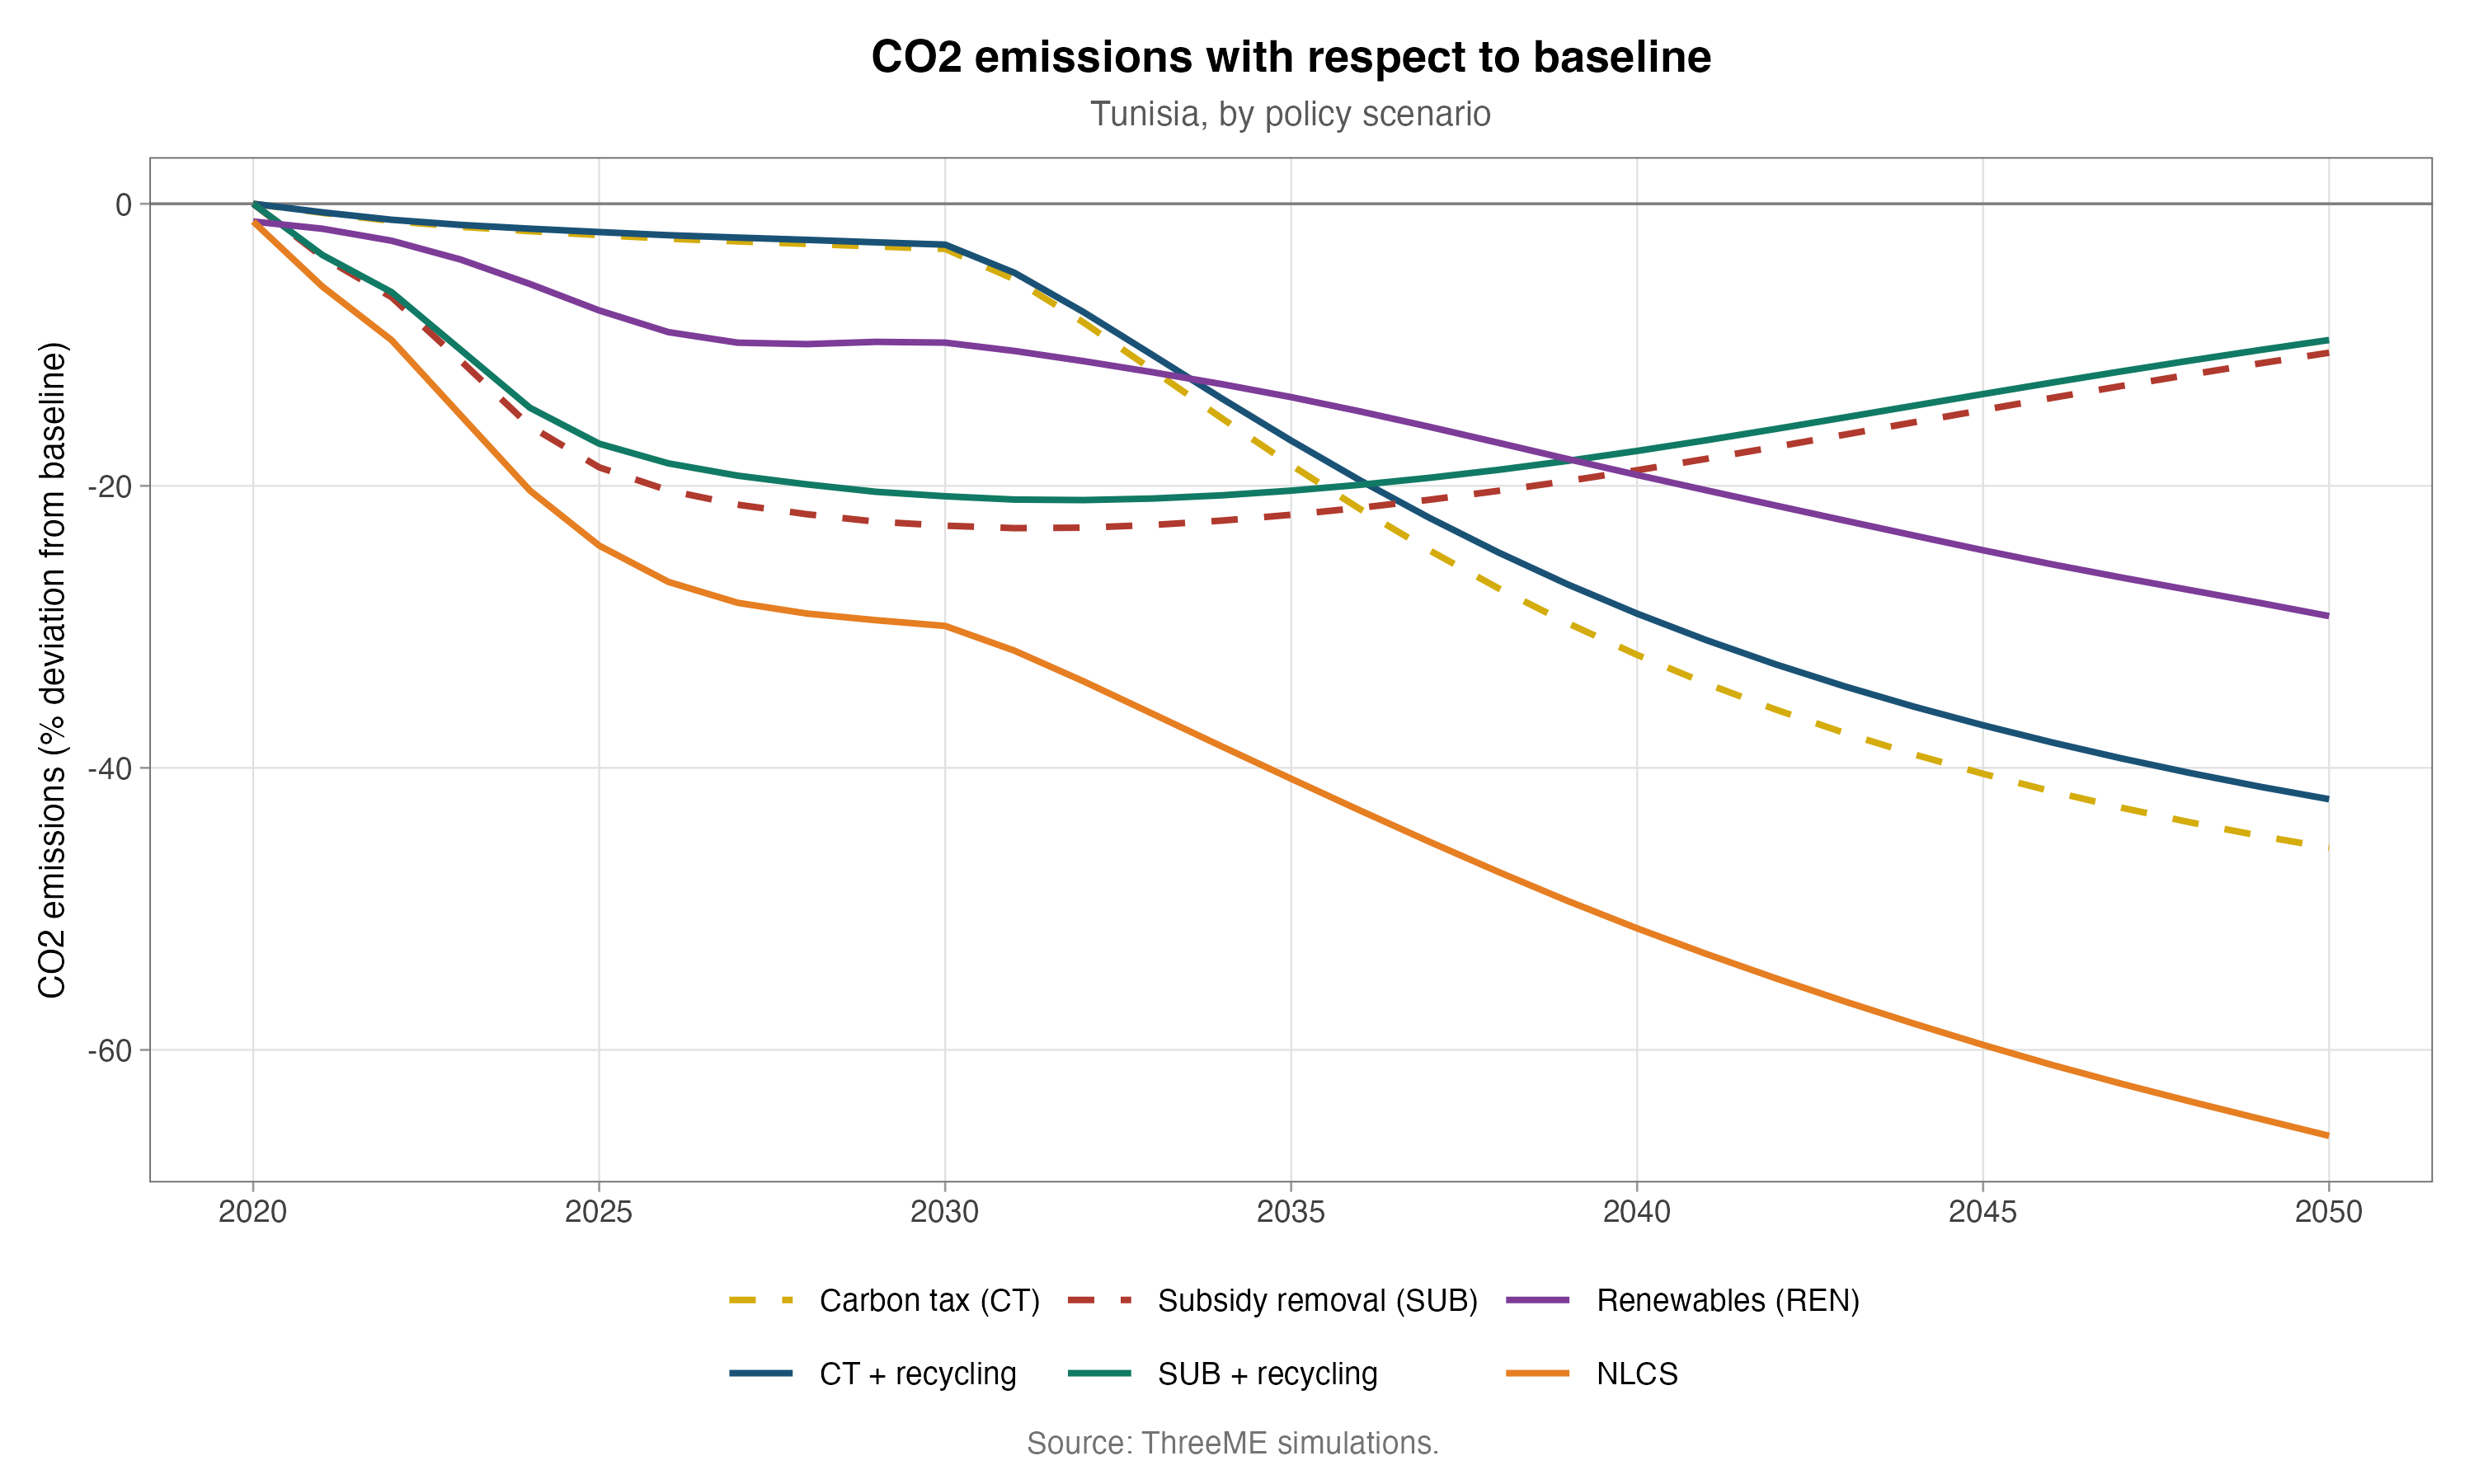
\includegraphics[width=0.95\textwidth]{fig01_co2_scenarios_tunisie.png}
    \caption{Émissions de CO$_2$ selon les scénarios -- Tunisie (avec et sans recyclage)}
    \label{fig:co2_scenarios}
\end{figure}

Pour le volet environnemental, les scénarios avec et sans recyclage présentent des baisses des émissions comparables, quoique légèrement plus importantes pour les scénarios sans recyclage, ce qui s'explique par une activité économique plus faible (Figure~\ref{fig:co2_scenarios}).

\begin{figure}[H]
    \centering
    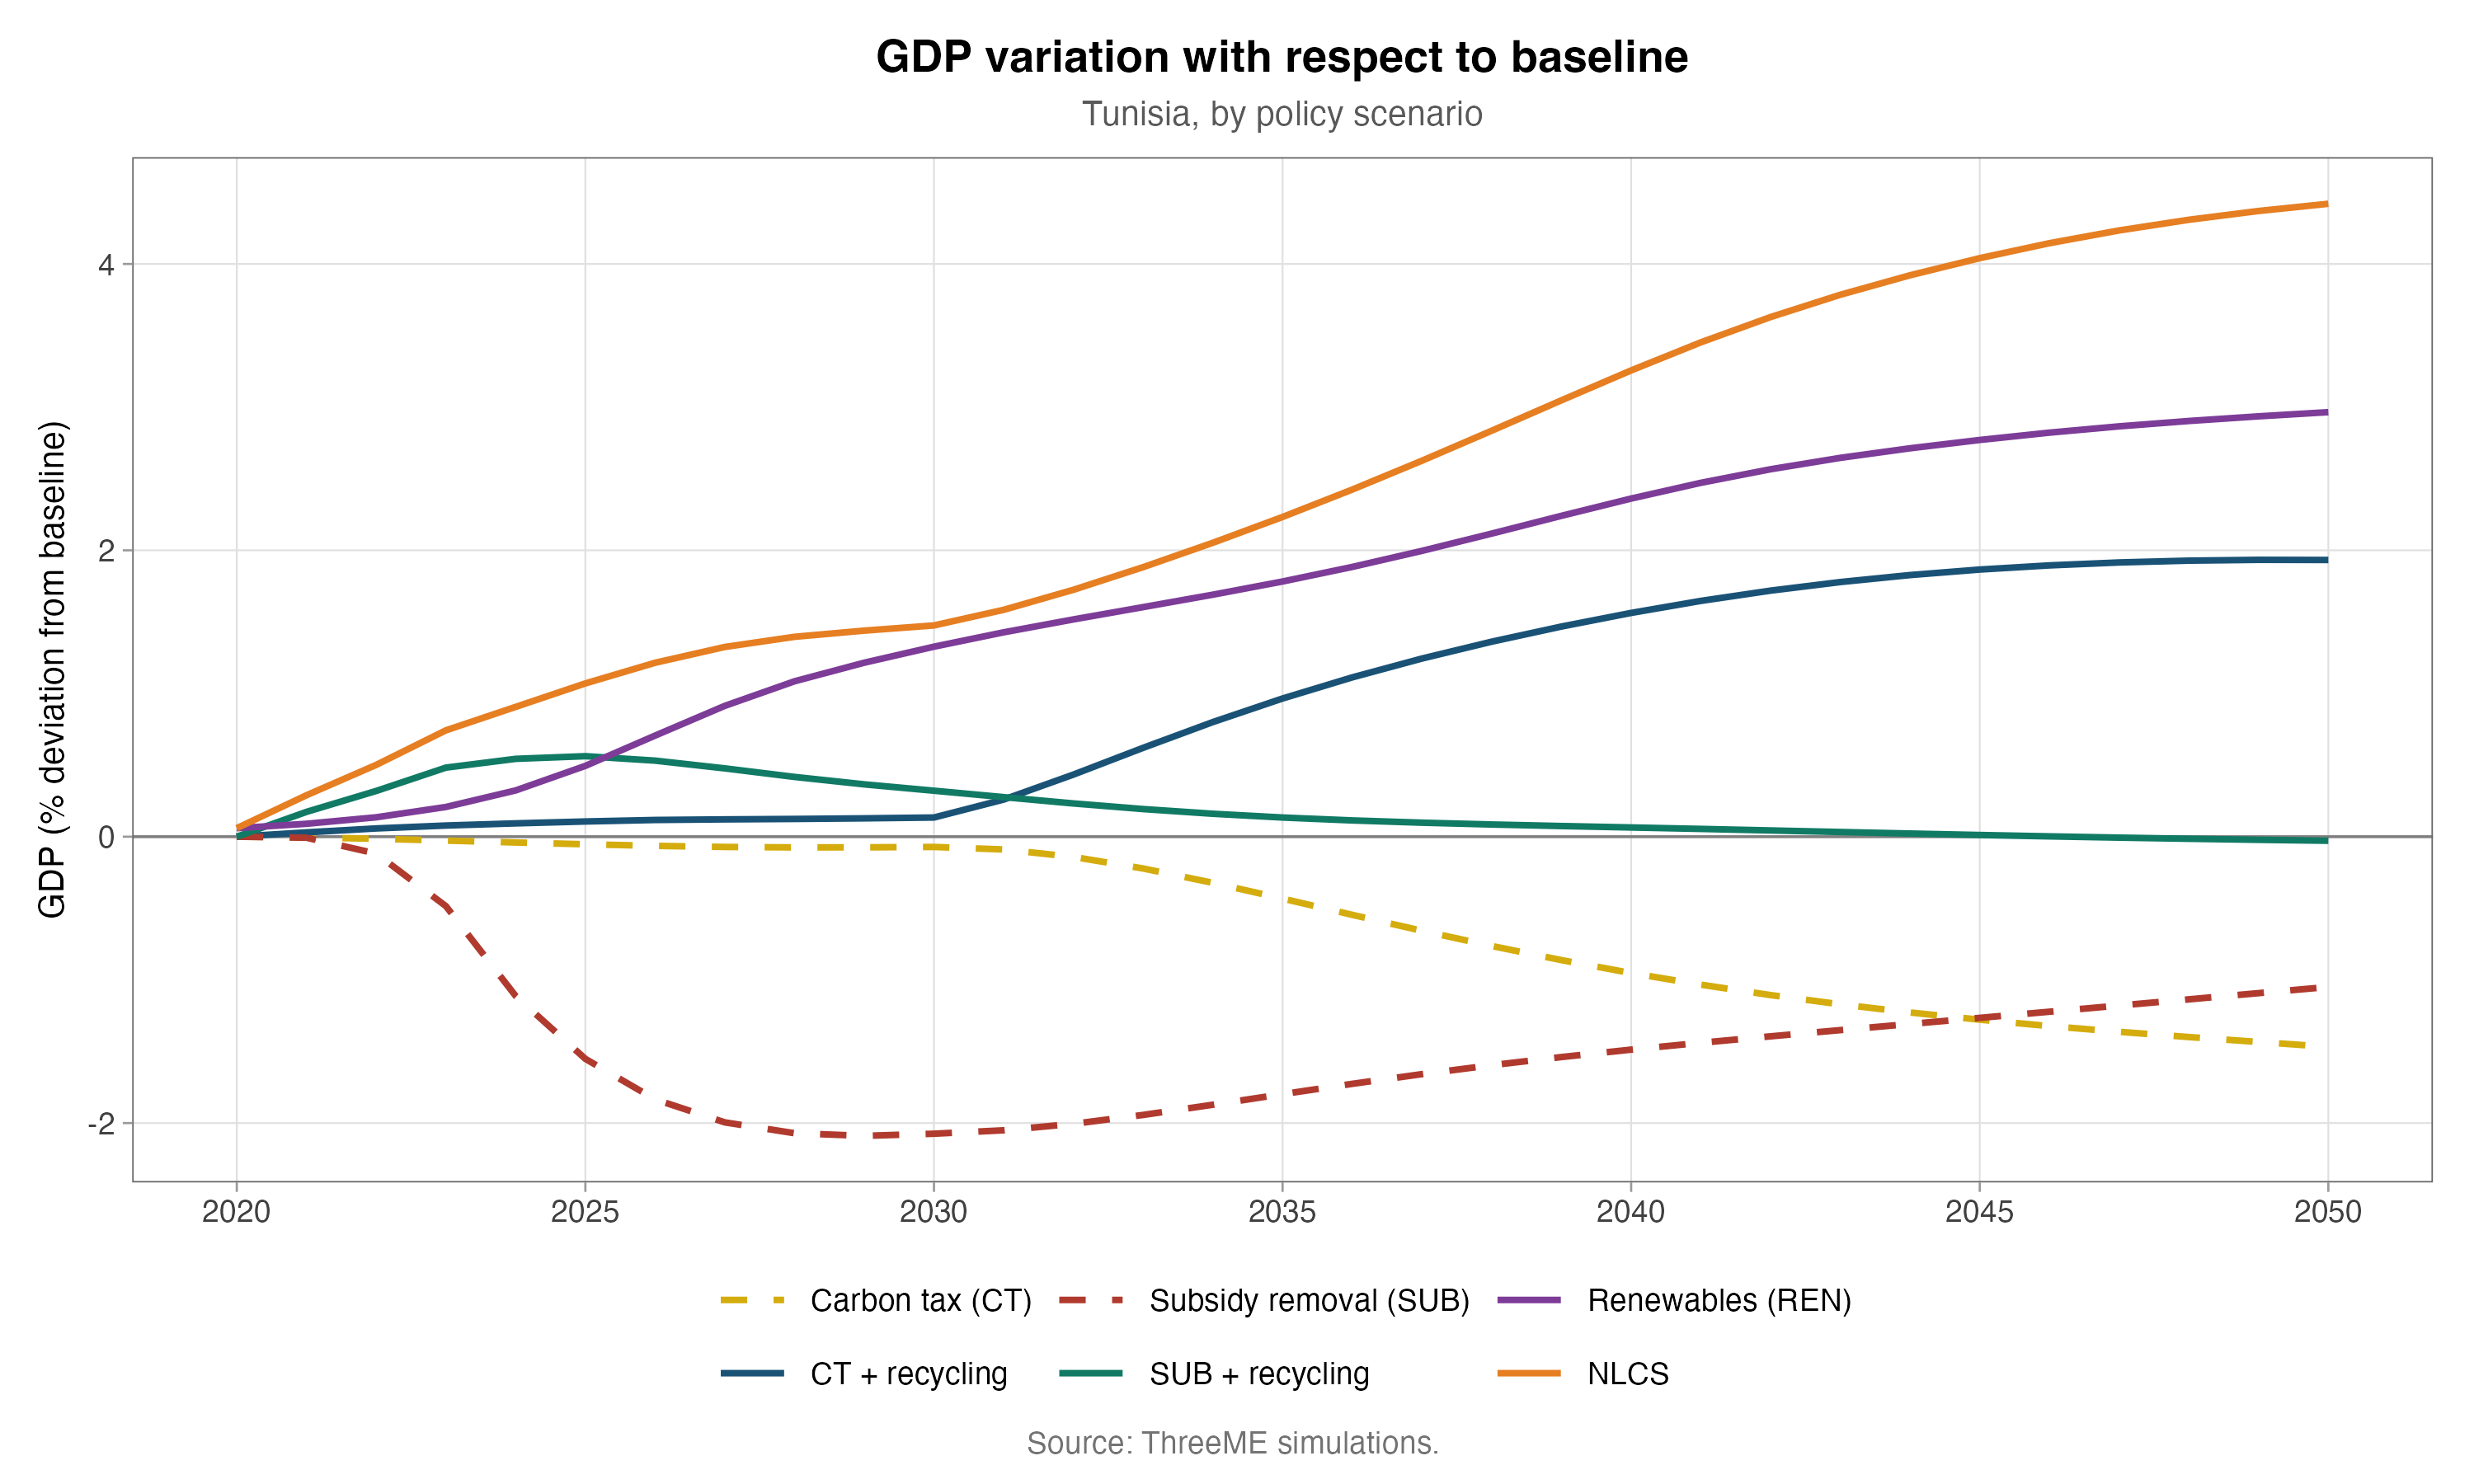
\includegraphics[width=0.95\textwidth]{fig02_pib_scenarios_tunisie.png}
    \caption{PIB selon les scénarios -- Tunisie (avec et sans recyclage)}
    \label{fig:gdp_scenarios}
\end{figure}

Concernant le volet économique, les scénarios avec recyclage affichent des indicateurs macroéconomiques nettement plus performants que leurs équivalents sans recyclage (Figure~\ref{fig:gdp_scenarios}). Le PIB est en dessous du niveau de la baseline dans le scénario sans recyclage et au-dessus avec recyclage. Ainsi, le dividende économique des mesures fiscales bas carbone apparaît grâce au recyclage. L'analyse des impacts agrégés et sectoriels confirme que le recyclage des recettes est une condition nécessaire à l'obtention d'un double dividende dans le contexte tunisien. La suite de cet article propose une comparaison de scénarios nationaux avec recyclage intégral des revenus de la fiscalité carbone.

% ========================================
% 4. ANALYSE COMPARATIVE TUNISIE-MEXIQUE
% ========================================
\section{Analyse comparative : transition en Tunisie et au Mexique}
\label{sec:comparaison}

Dans cette section, nous proposons une approche comparée des stratégies de transition énergétique en Tunisie et au Mexique. Il s'agit dans les deux cas de simulations de scénarios de politiques de transition pour des pays en développement utilisant le modèle ThreeME, réalisées en collaboration avec des parties prenantes locales et ayant donné lieu à la création de modèles nationaux originaux paramétrés avec des données spécifiques à chaque pays.

Si les économies tunisienne et mexicaine sont très différentes, les exercices de simulation présentent des similarités intéressantes : le taux de collecte de taxe carbone dans le PIB atteint un niveau proche entre 2 et 3 points de PIB en 2050, le prix du carbone atteint respectivement 132 et 135~\$/tCO$_2$, et la pénétration des énergies renouvelables dans le mix électrique est importante, à hauteur de 80\,\% en Tunisie et de 50\,\% au Mexique.

\subsection{Trajectoires de tarification carbone}

\begin{figure}[H]
    \centering
    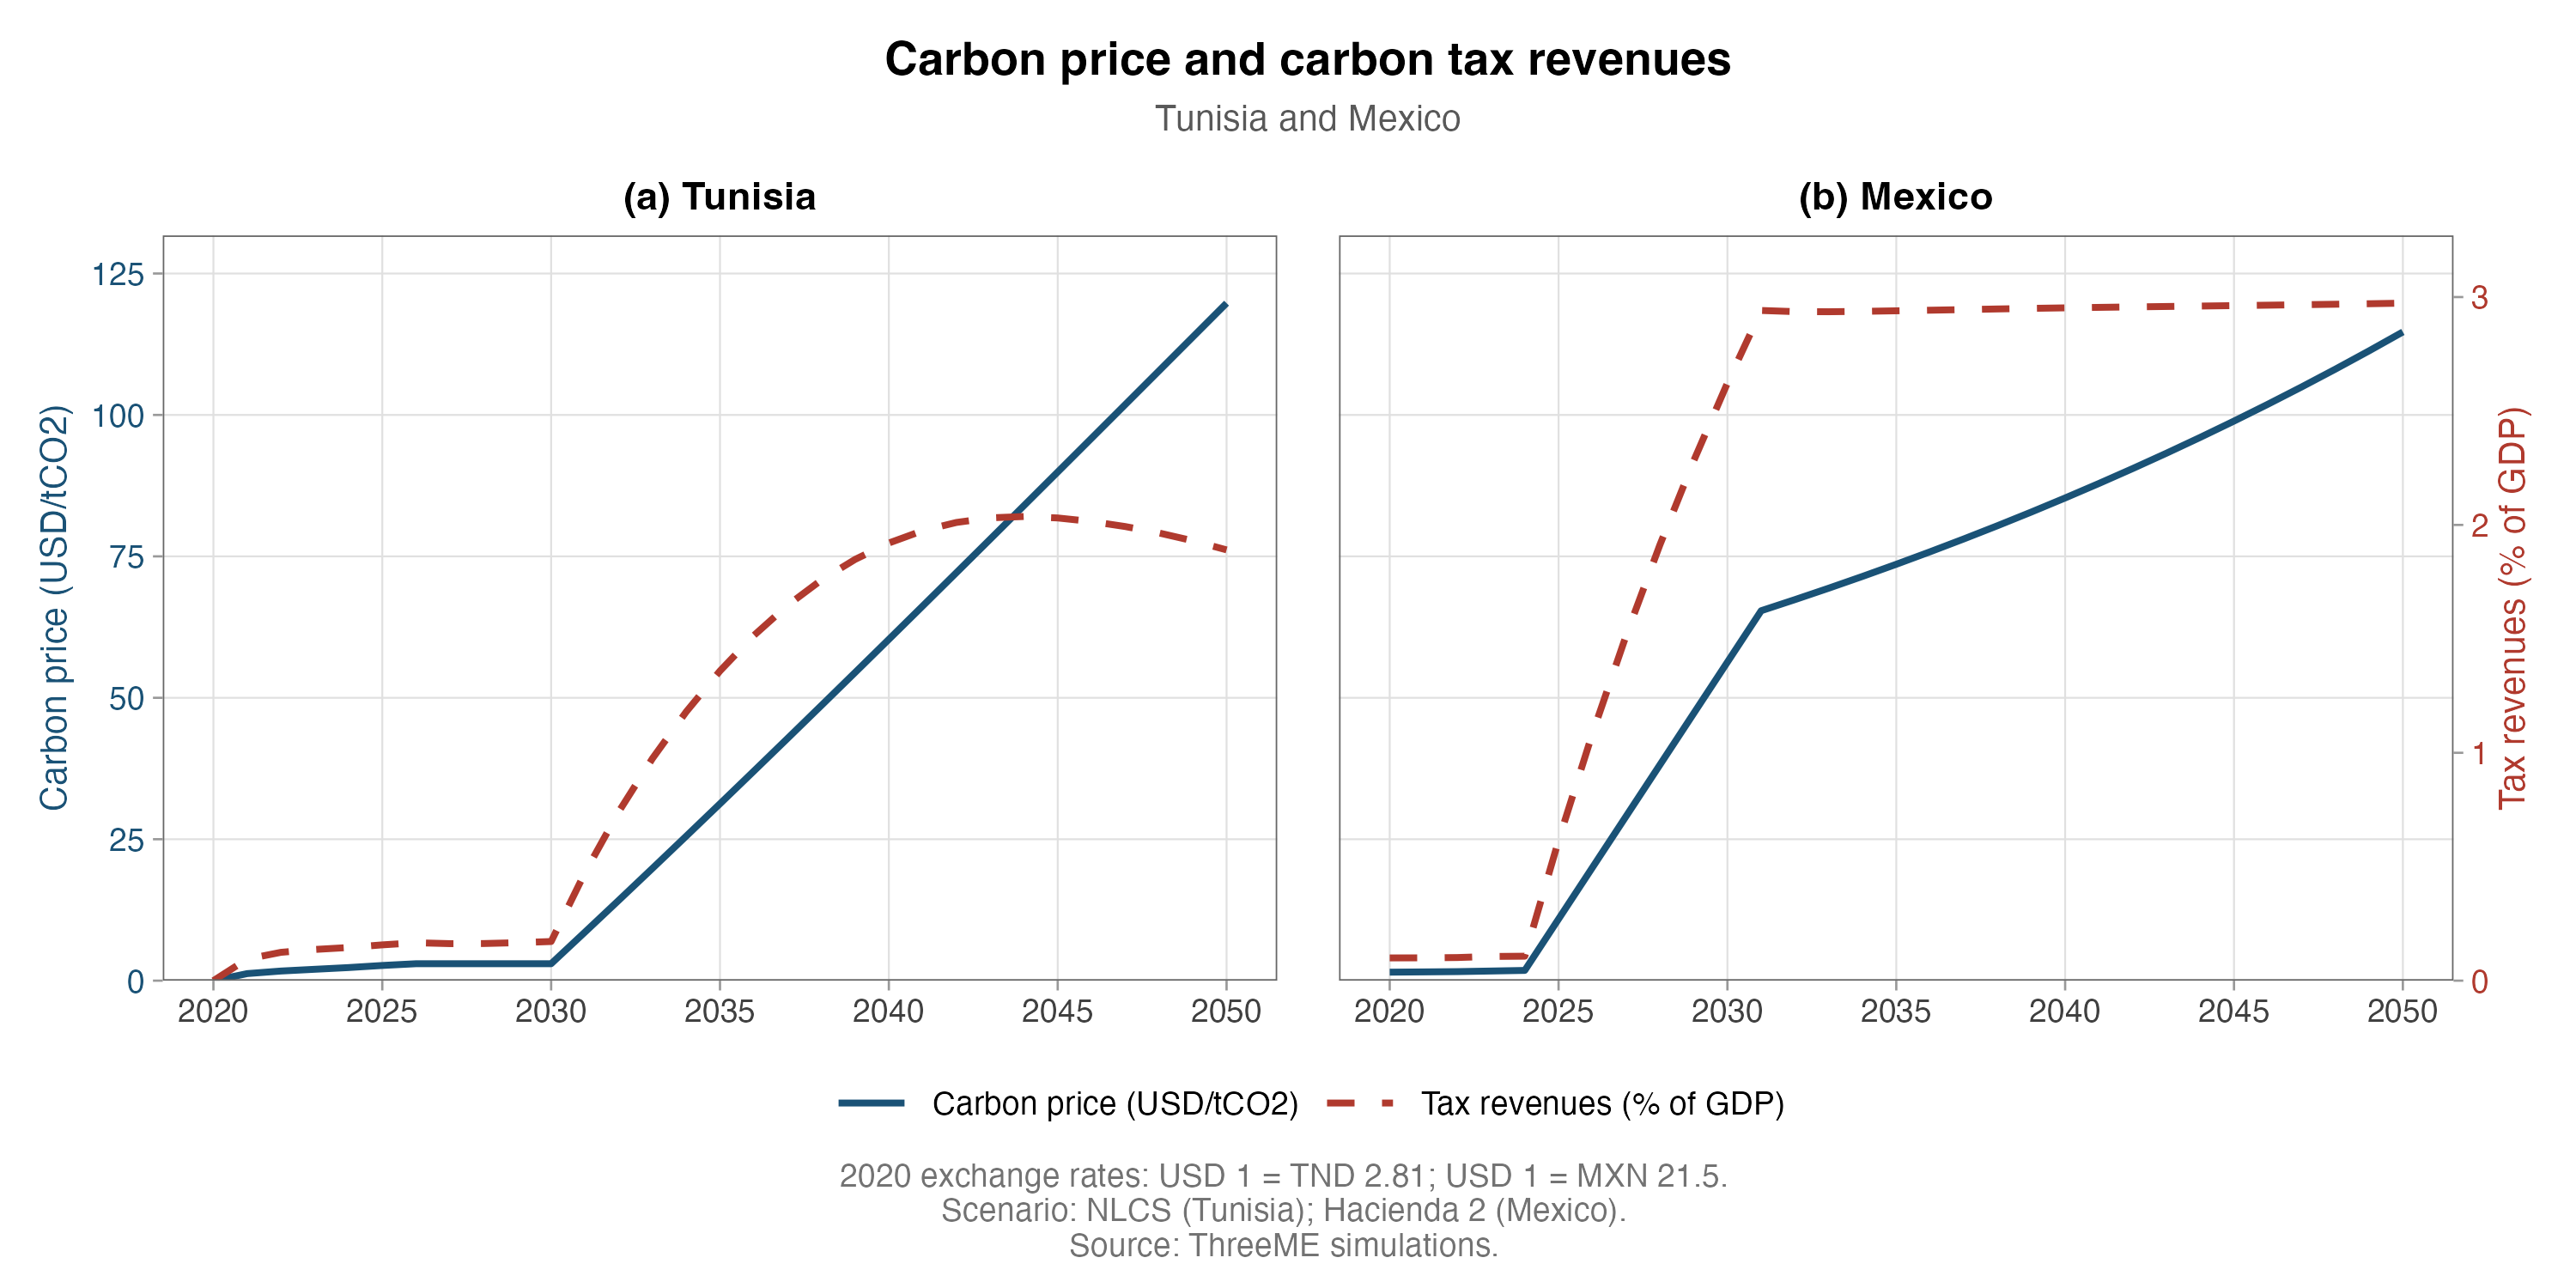
\includegraphics[width=0.95\textwidth]{fig03_taxe_carbone.png}
    \caption{Comparaison des trajectoires de taxe carbone -- Tunisie et Mexique}
    \label{fig:carbon_tax}
\end{figure}

La figure~\ref{fig:carbon_tax} montre que si les niveaux de taxe carbone sont comparables en 2050, les trajectoires diffèrent : la taxe carbone augmente plus rapidement au Mexique autour de 2030, là où elle n'atteint un niveau similaire qu'environ 10 ans plus tard dans le scénario tunisien. Cette différence de rythme a des implications importantes sur les dynamiques de court et moyen terme, comme nous le verrons dans l'analyse des résultats.

\subsection{Efficacité environnementale et découplage}

Les stratégies de transition atteignent leur objectif dans les deux pays. À l'horizon 2050, les émissions baissent d'environ 60\,\% pour la Tunisie et 50\,\% pour le Mexique par rapport à leurs scénarios de référence respectifs. Cette baisse, conjuguée à une hausse du PIB, permet d'observer un découplage entre croissance et émissions (Figure~\ref{fig:decoupling}).

\begin{figure}[H]
    \centering
    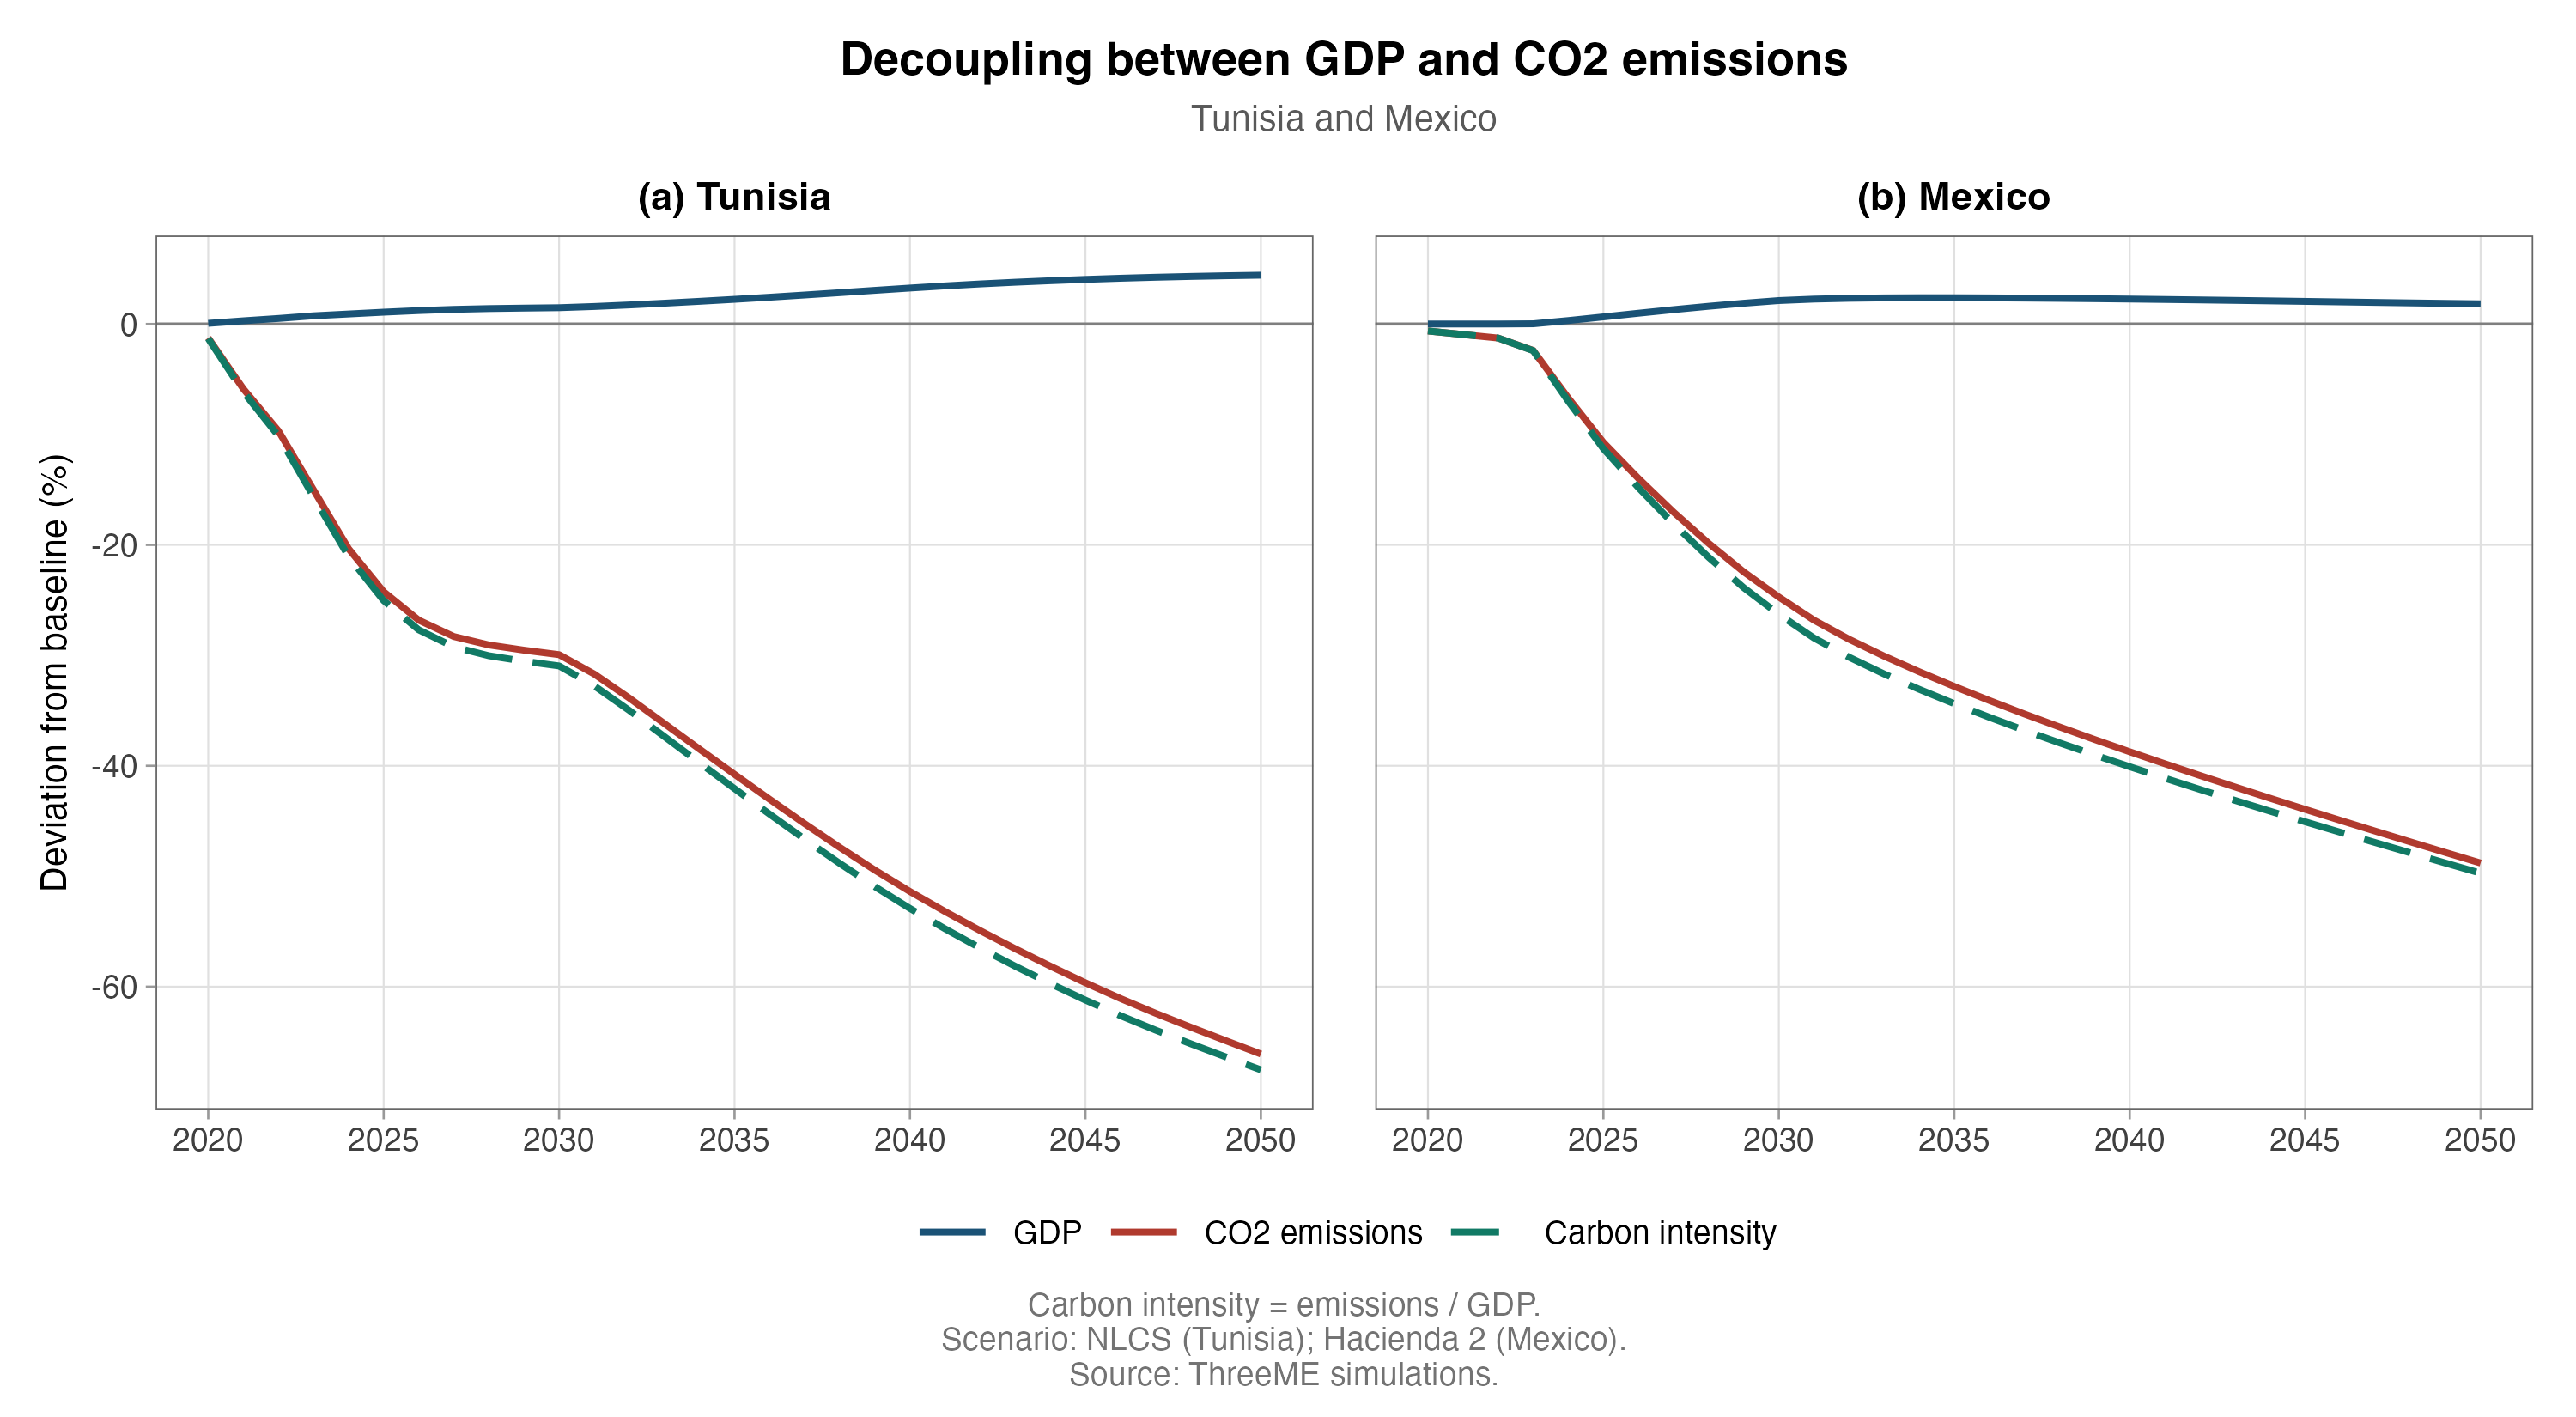
\includegraphics[width=0.95\textwidth]{fig04_decouplage.png}
    \caption{Découplage entre croissance économique et émissions de CO$_2$}
    \label{fig:decoupling}
\end{figure}

\subsection{Effets macroéconomiques agrégés : un choc asymétrique}

\begin{figure}[H]
    \centering
    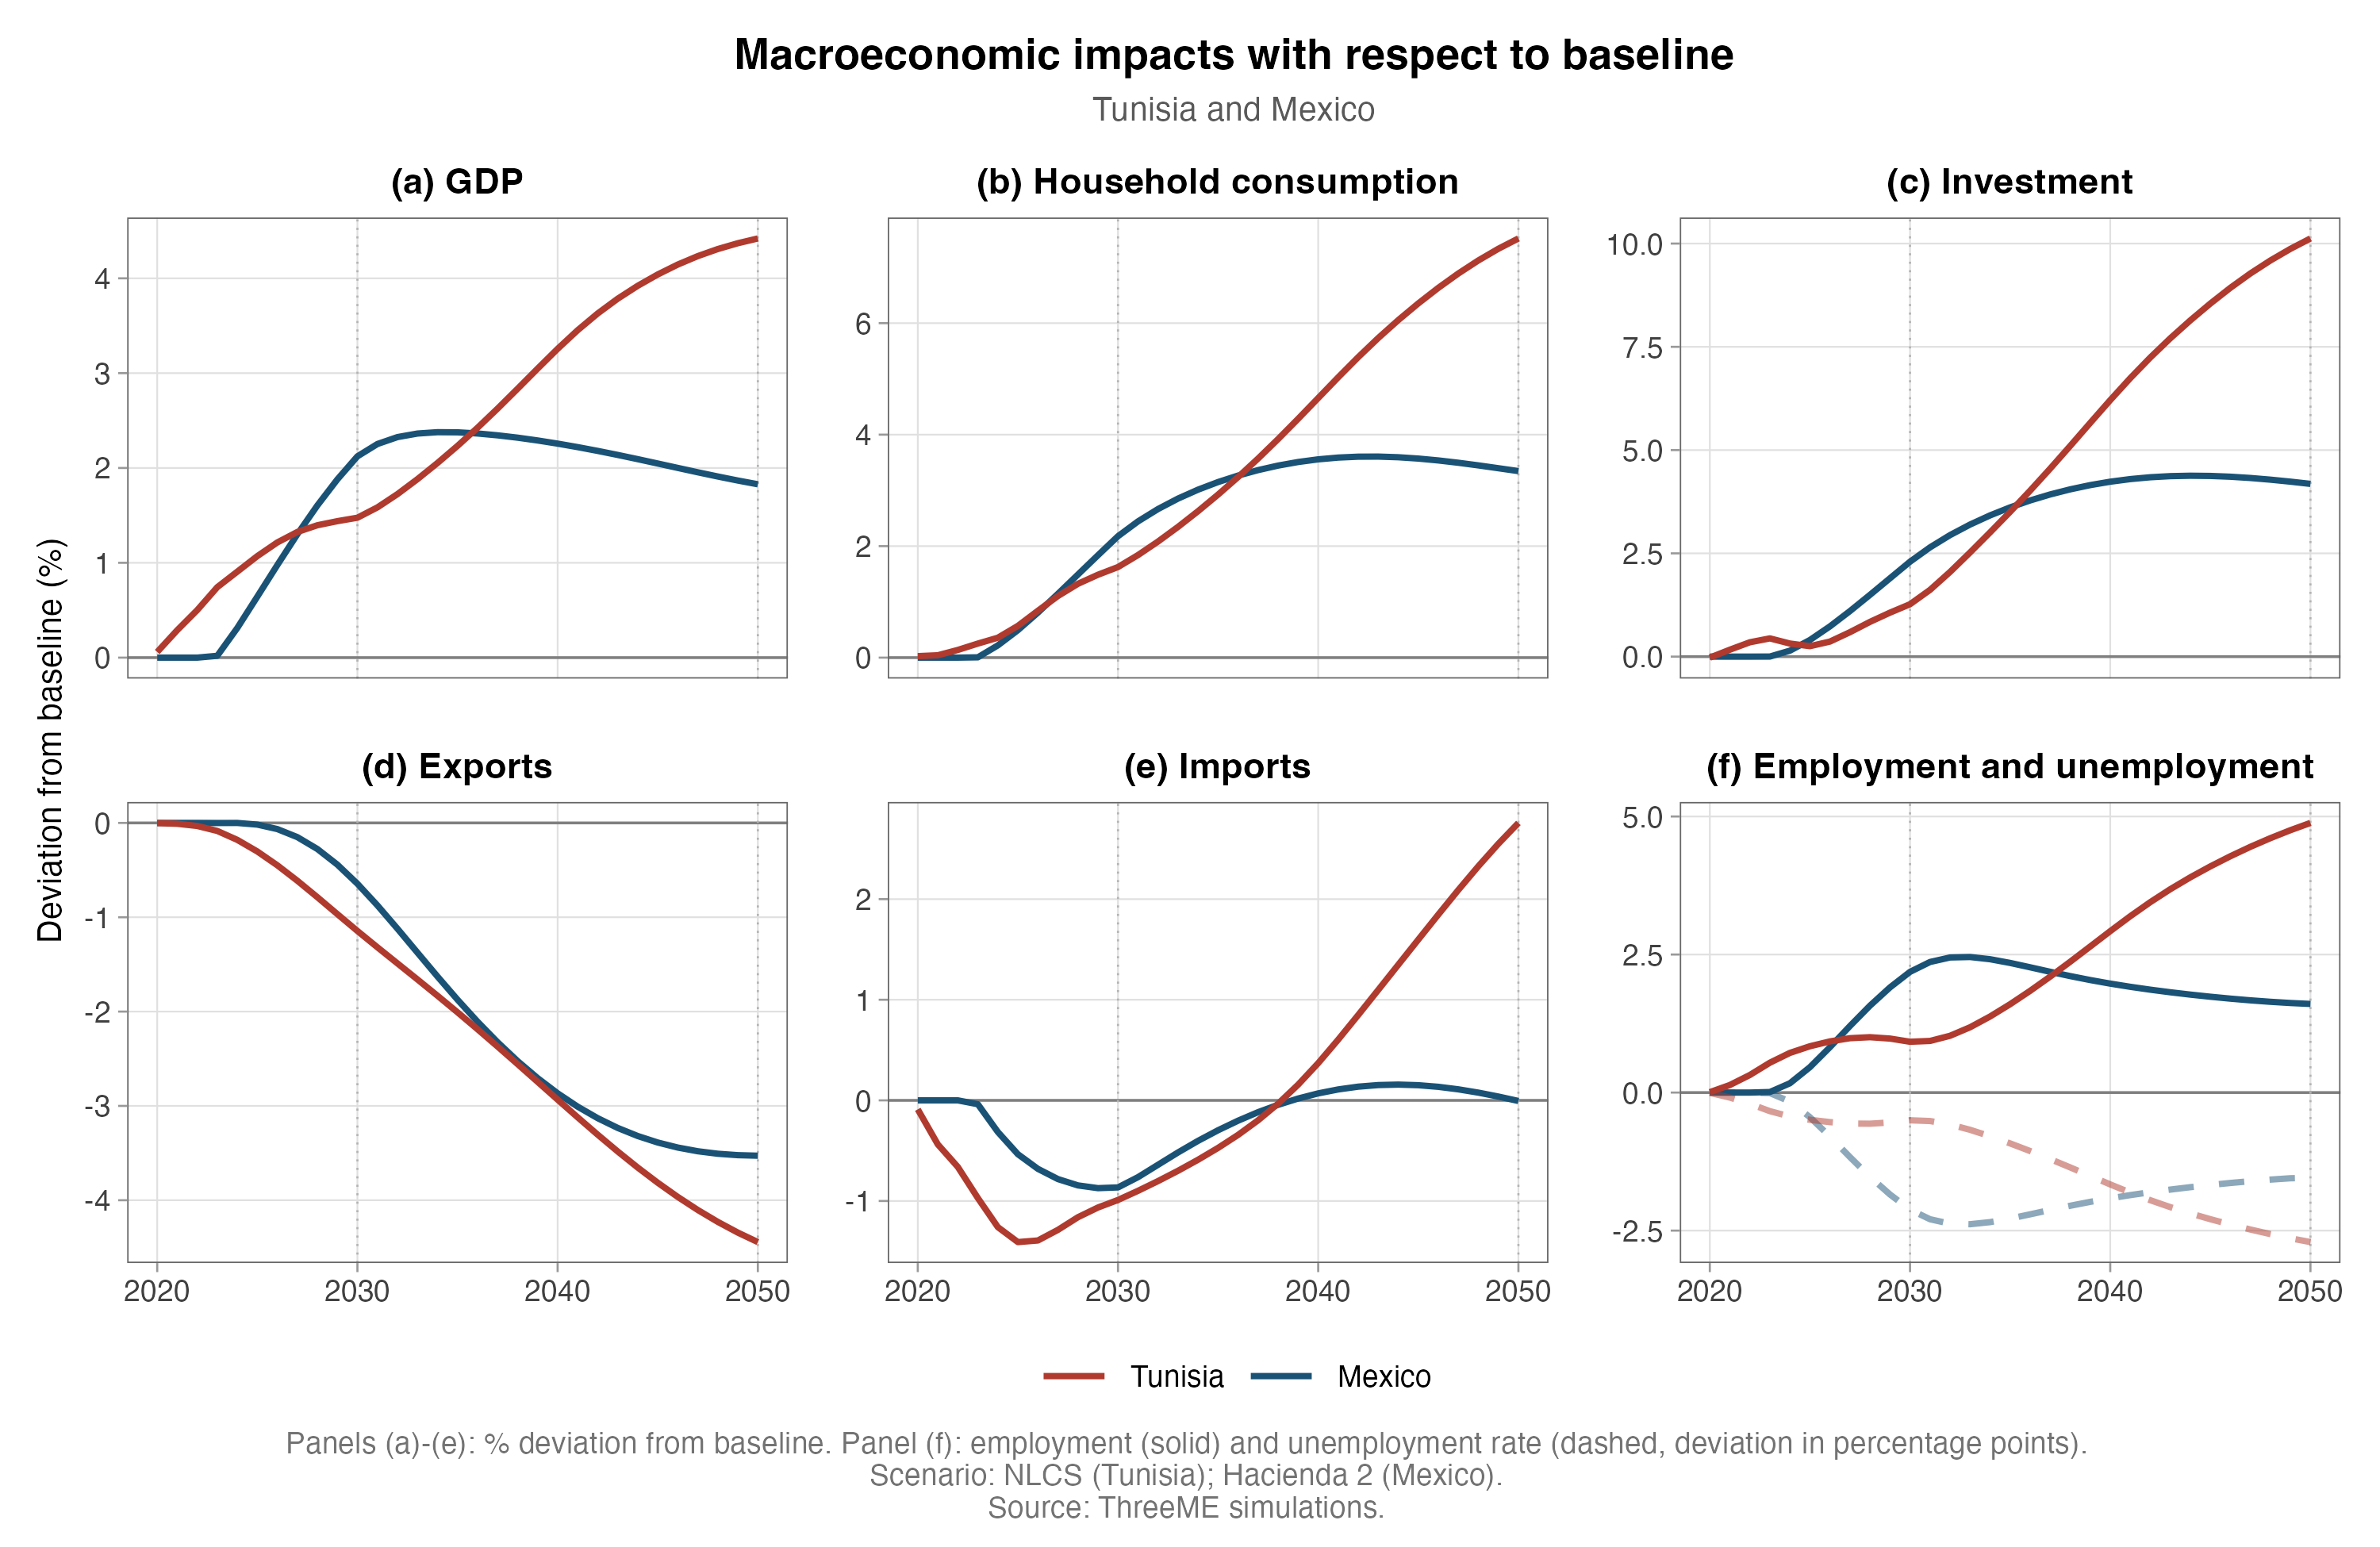
\includegraphics[width=0.95\textwidth]{fig05_impact_macro.png}
    \caption{Impact macroéconomique comparé -- Tunisie et Mexique (écarts au scénario de référence en 2030 et 2050)}
    \label{fig:macro_impact}
\end{figure}

La comparaison des grands indicateurs macroéconomiques (Figure~\ref{fig:macro_impact}) montre qu'à l'horizon 2050, le \textit{policy mix} tunisien génère des gains plus importants par rapport à la baseline que celui mené au Mexique. Nous l'expliquons par trois arguments clés.

\textbf{Premièrement, le caractère asymétrique du choc selon la structure énergétique.} En Tunisie, pays importateur net d'hydrocarbures, la tarification du carbone et la montée des renouvelables réduisent progressivement la demande énergétique extérieure, remplacée par la production électrique domestique. La baisse des importations d'énergie fossile améliore la balance commerciale et relocalise une partie de la dépense énergétique vers l'investissement et la production des secteurs moins carbonés. La transition agit ainsi comme un choc de demande positif, soutenu par l'investissement vert et les effets multiplicateurs associés : l'investissement dans les infrastructures ENR agit comme un plan de relance.

Au Mexique, la transition se traduit par un choc d'offre négatif sur un secteur exportateur clé. La taxe carbone entraîne une baisse de la demande agrégée pour le secteur de l'énergie. La compétitivité et la rentabilité du secteur pétrolier diminuent, entraînant une contraction de la production fossile et une réallocation du capital et du travail vers d'autres secteurs. Si les renouvelables et les services se développent, cette expansion ne compense que progressivement la perte de valeur ajoutée dans l'extractif.

\textbf{Deuxièmement, l'importance de la situation macroéconomique initiale.} La Tunisie, dans une trajectoire de croissance sous-optimale marquée par un taux de chômage élevé, dispose de facteurs de production inemployés. Le surcroît d'investissement et de demande associé à la transition s'apparente à un keynésianisme vert qui amplifie les effets positifs sur le PIB, la consommation et l'emploi. Pour le Mexique, plus proche du plein emploi, le multiplicateur keynésien est plus fortement limité par la disponibilité des facteurs de production.

\textbf{Troisièmement, la dimension temporelle et le signal-prix.} La hausse plus rapide de la taxe au Mexique accélère le déclin relatif du secteur pétrolier et accentue les besoins de réallocation sectorielle, pesant davantage sur la dynamique macroéconomique à moyen terme. En Tunisie, la première phase est principalement marquée par l'effet de l'investissement dans les ENR, avec une augmentation progressive du signal-prix qui renforce la substitution aux importations fossiles.

\subsection{Décomposition du PIB par composantes de la demande}
\label{subsec:decomposition_pib}

Afin de comprendre les mécanismes sous-jacents à la dynamique du PIB, nous analysons les contributions de chaque composante de la demande finale à la variation du PIB par rapport au scénario de référence (Figure~\ref{fig:decomp_pib}).

\begin{figure}[H]
    \centering
    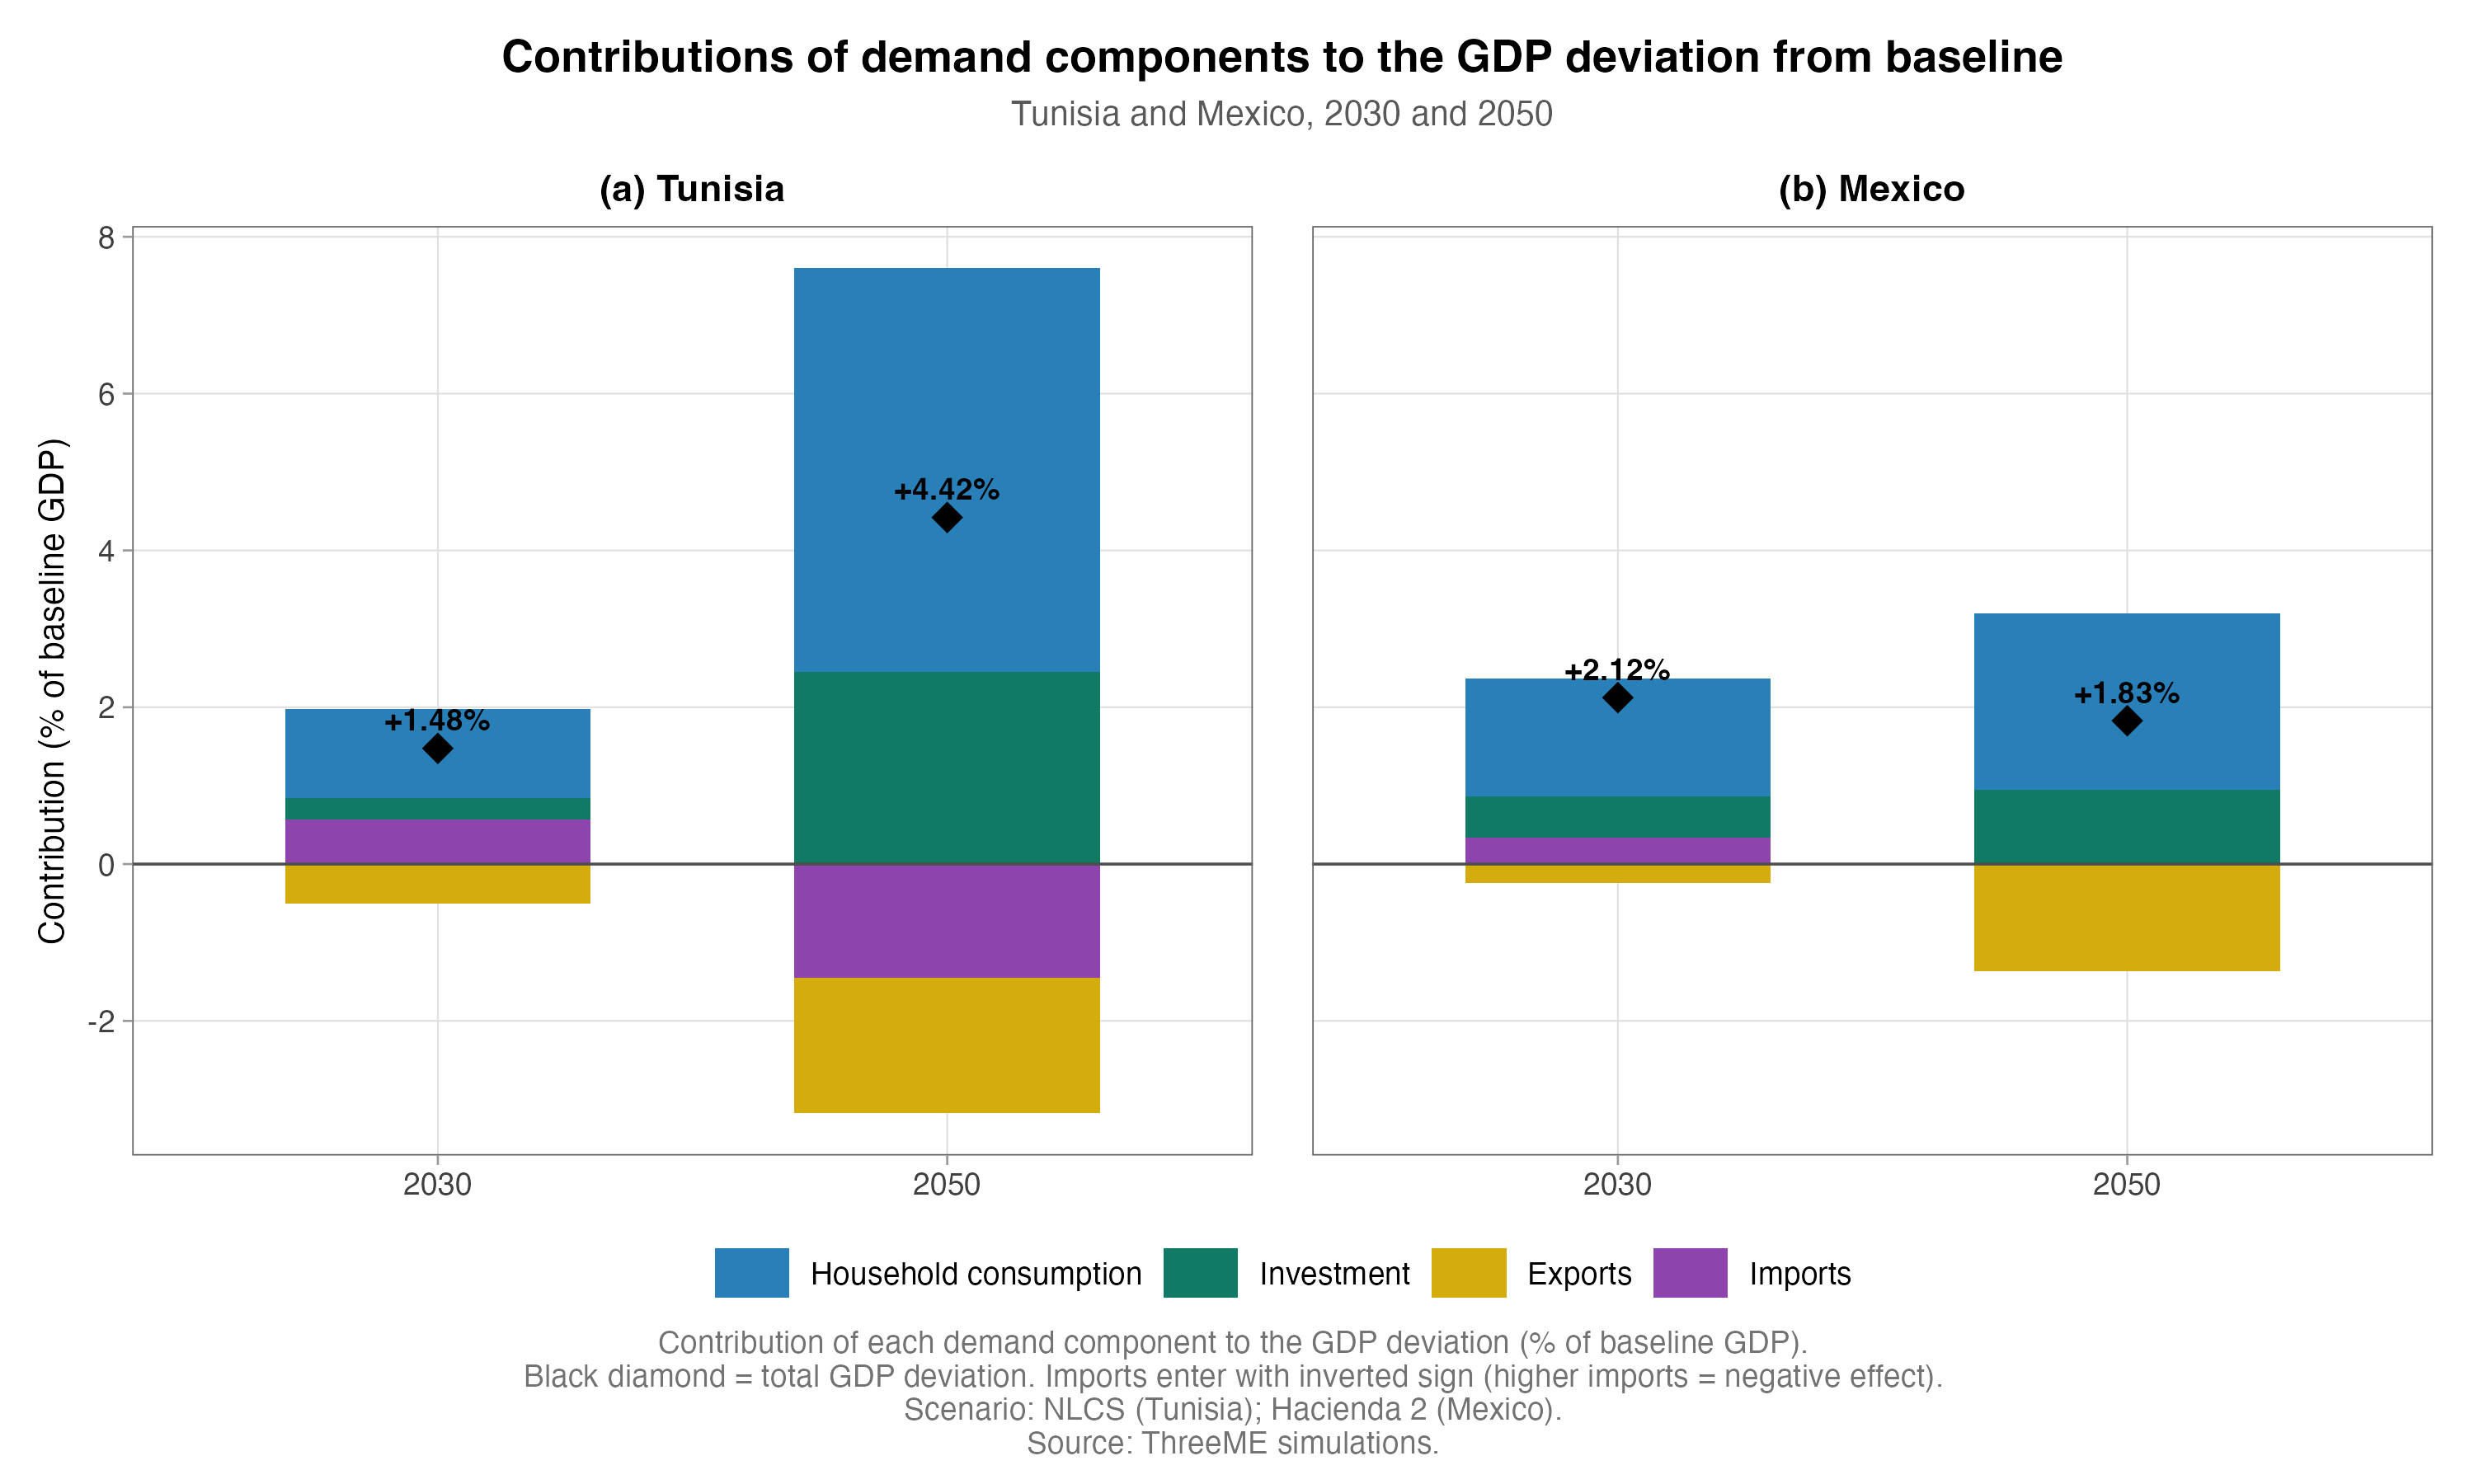
\includegraphics[width=0.95\textwidth]{fig08_decomposition_pib.png}
    \caption{Décomposition du PIB par composantes de la demande -- Tunisie (SNBC) et Mexique (en 2030 et 2050)}
    \label{fig:decomp_pib}
\end{figure}

Pour la Tunisie, dans le scénario SNBC, les effets positifs l'emportent nettement. La consommation des ménages et l'investissement productif constituent les principaux moteurs de la croissance, compensant la contribution négative de la balance commerciale. Le PIB tunisien augmente de 1\,\% dès 2025, puis de 2,13\,\% en 2035, pour aller jusqu'à atteindre +5\,\% à l'horizon 2050 par rapport au scénario de référence. Cette progression soutenue traduit une dynamique robuste portée par la consommation des ménages et l'investissement productif, qui compensent les tensions extérieures générées par la dégradation de la balance commerciale.

Pour le Mexique, l'investissement joue également un rôle moteur, mais la contribution négative des exportations nettes est plus prononcée, reflétant la perte de compétitivité du secteur fossile et les besoins accrus en importations de biens d'équipement.

\subsection{Dynamique de l'investissement}
\label{subsec:investissement}

L'un des effets macroéconomiques majeurs de la transition concerne l'investissement. Moteur central de la transformation du système productif, il réagit de manière différenciée selon les instruments de politique mis en \oe{}uvre, mais montre globalement une dynamique positive à long terme.

\begin{figure}[H]
    \centering
    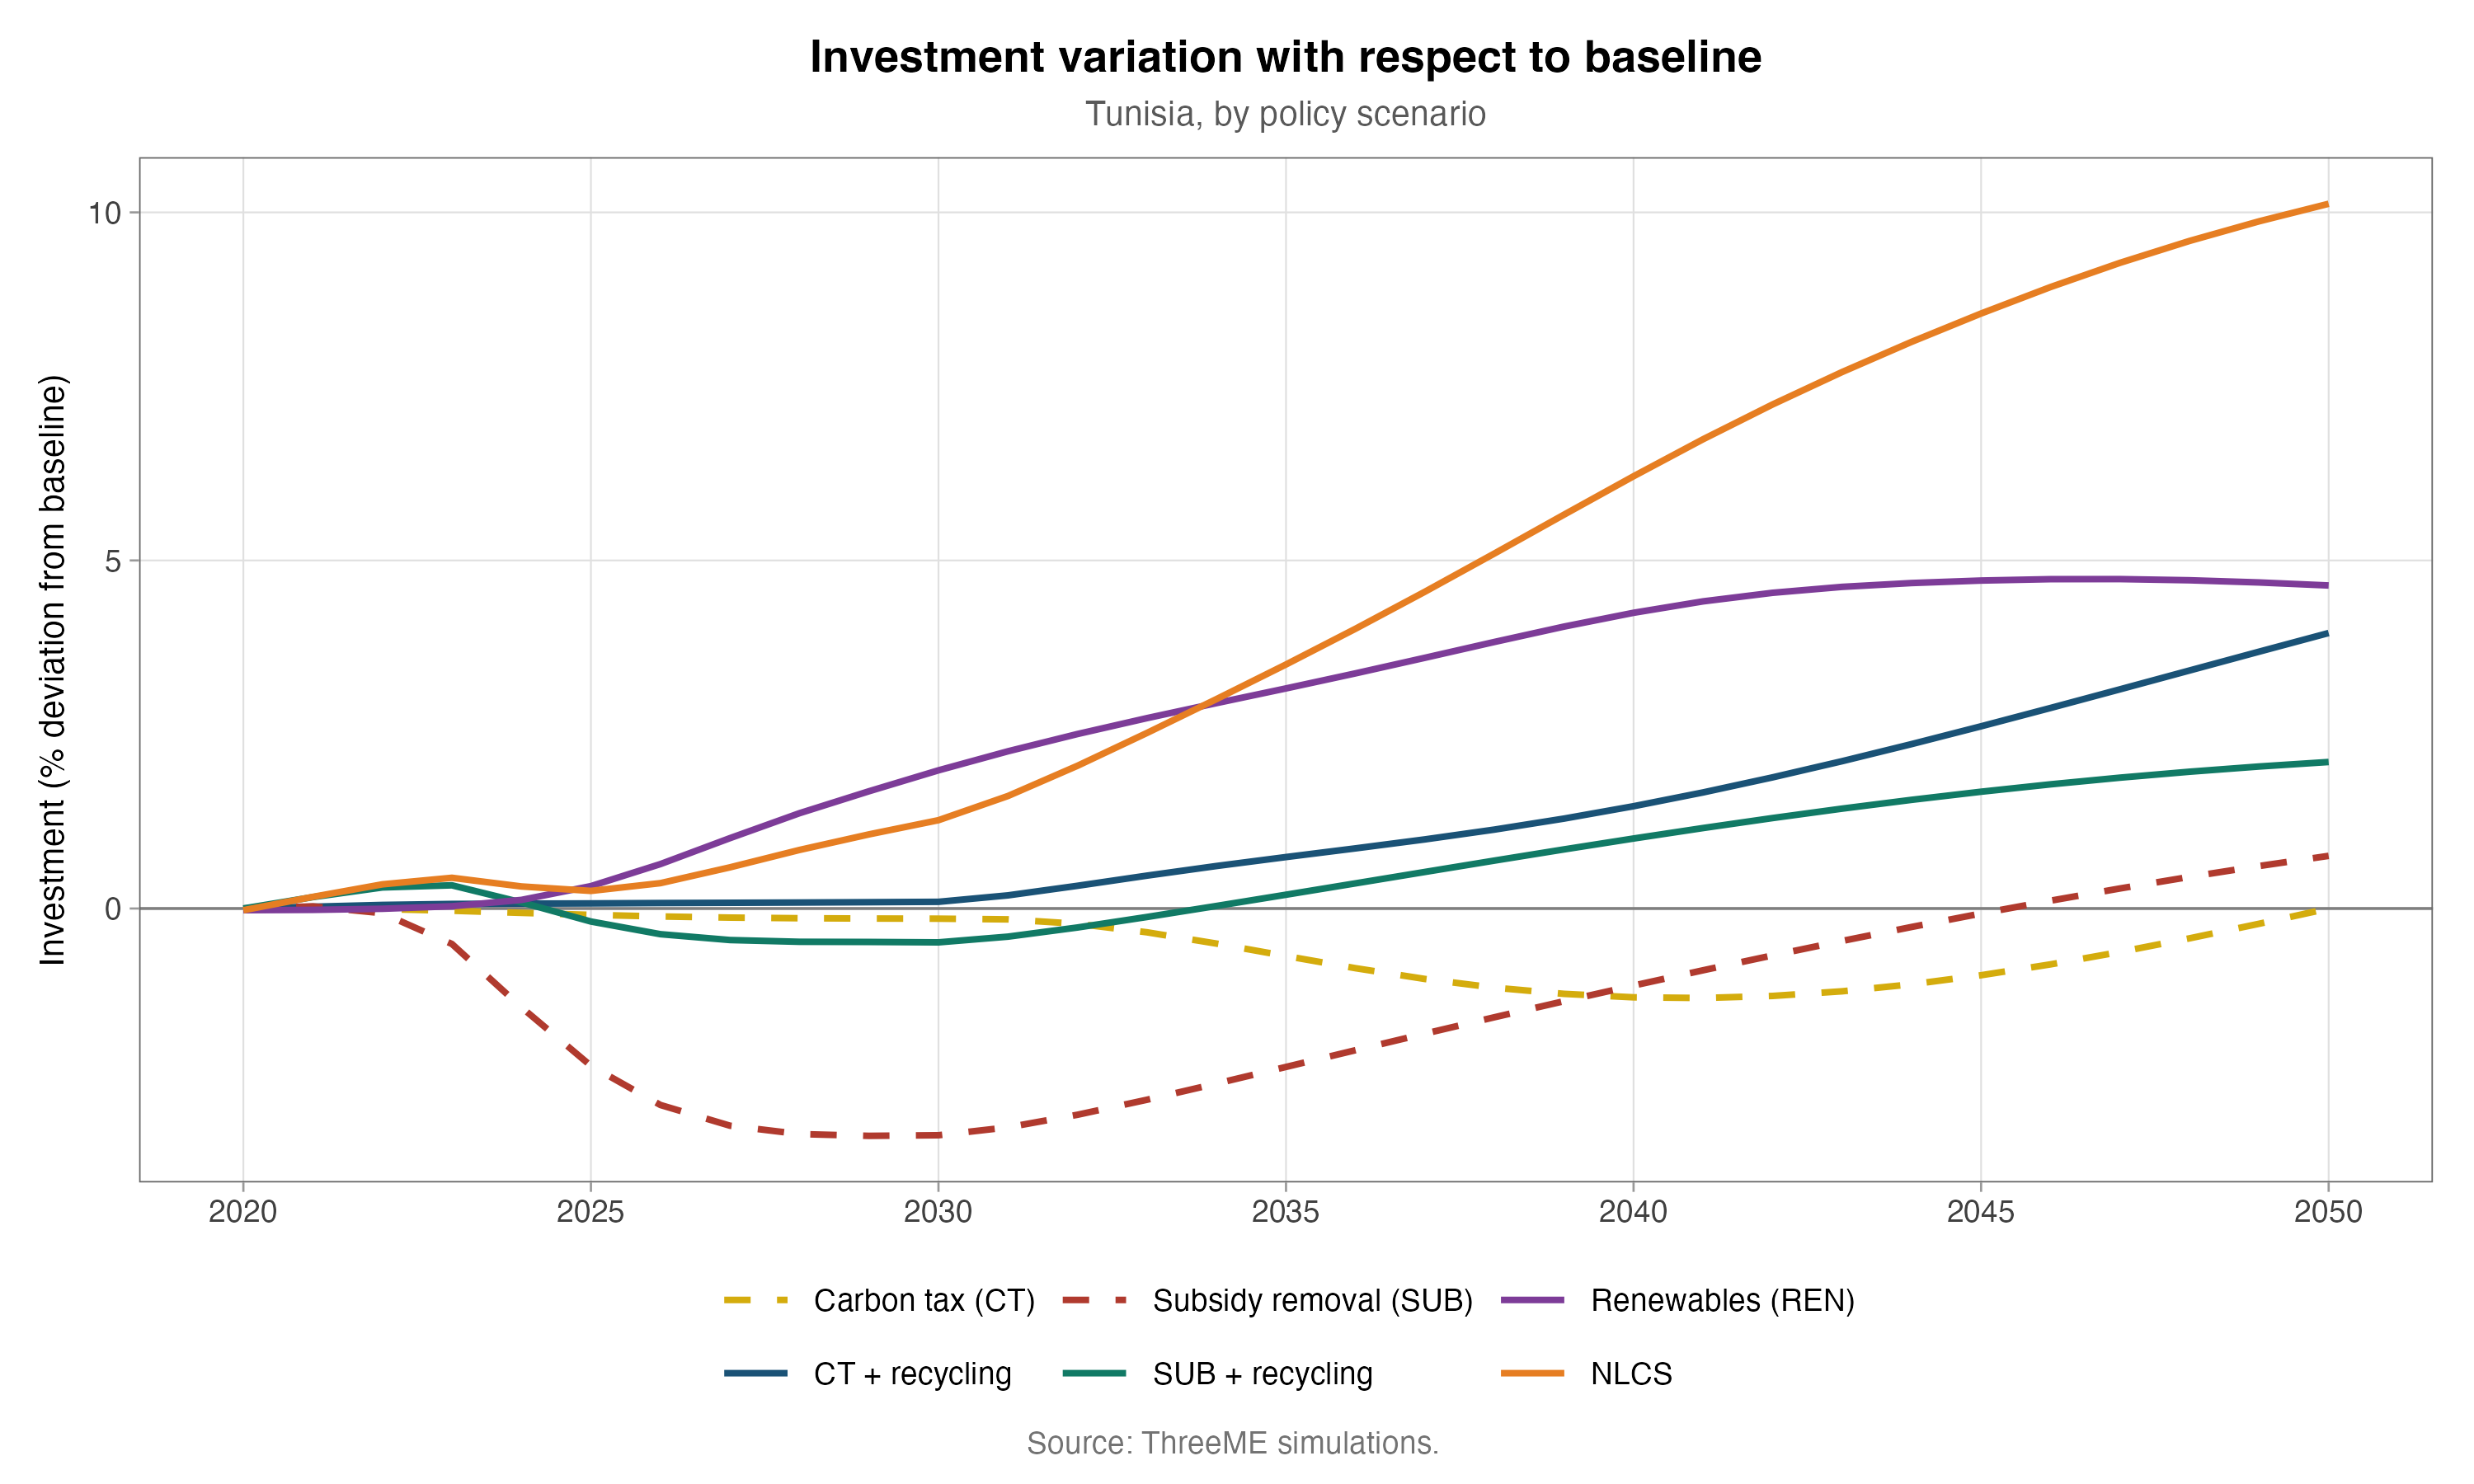
\includegraphics[width=0.95\textwidth]{fig09_investissement_scenarios.png}
    \caption{Variations relatives de l'investissement agrégé par scénario -- Tunisie}
    \label{fig:invest_scenarios}
\end{figure}

En Tunisie, les trajectoires observées pour l'investissement montrent une tendance similaire à celle de l'emploi (Figure~\ref{fig:invest_scenarios}). Dans les scénarios fondés sur le développement des énergies renouvelables, l'investissement progresse de manière régulière, principalement tiré par la construction d'infrastructures de production d'électricité renouvelable et la modernisation du réseau électrique. C'est dans le scénario SNBC complet que les effets les plus marquants sont observés : l'introduction d'une fiscalité carbone progressive, conjuguée à des signaux de prix incitatifs et au recyclage des recettes publiques, stimule significativement l'activité d'investissement. En 2050, l'investissement est supérieur de 12\,\% à celui du scénario de référence.

\begin{figure}[H]
    \centering
    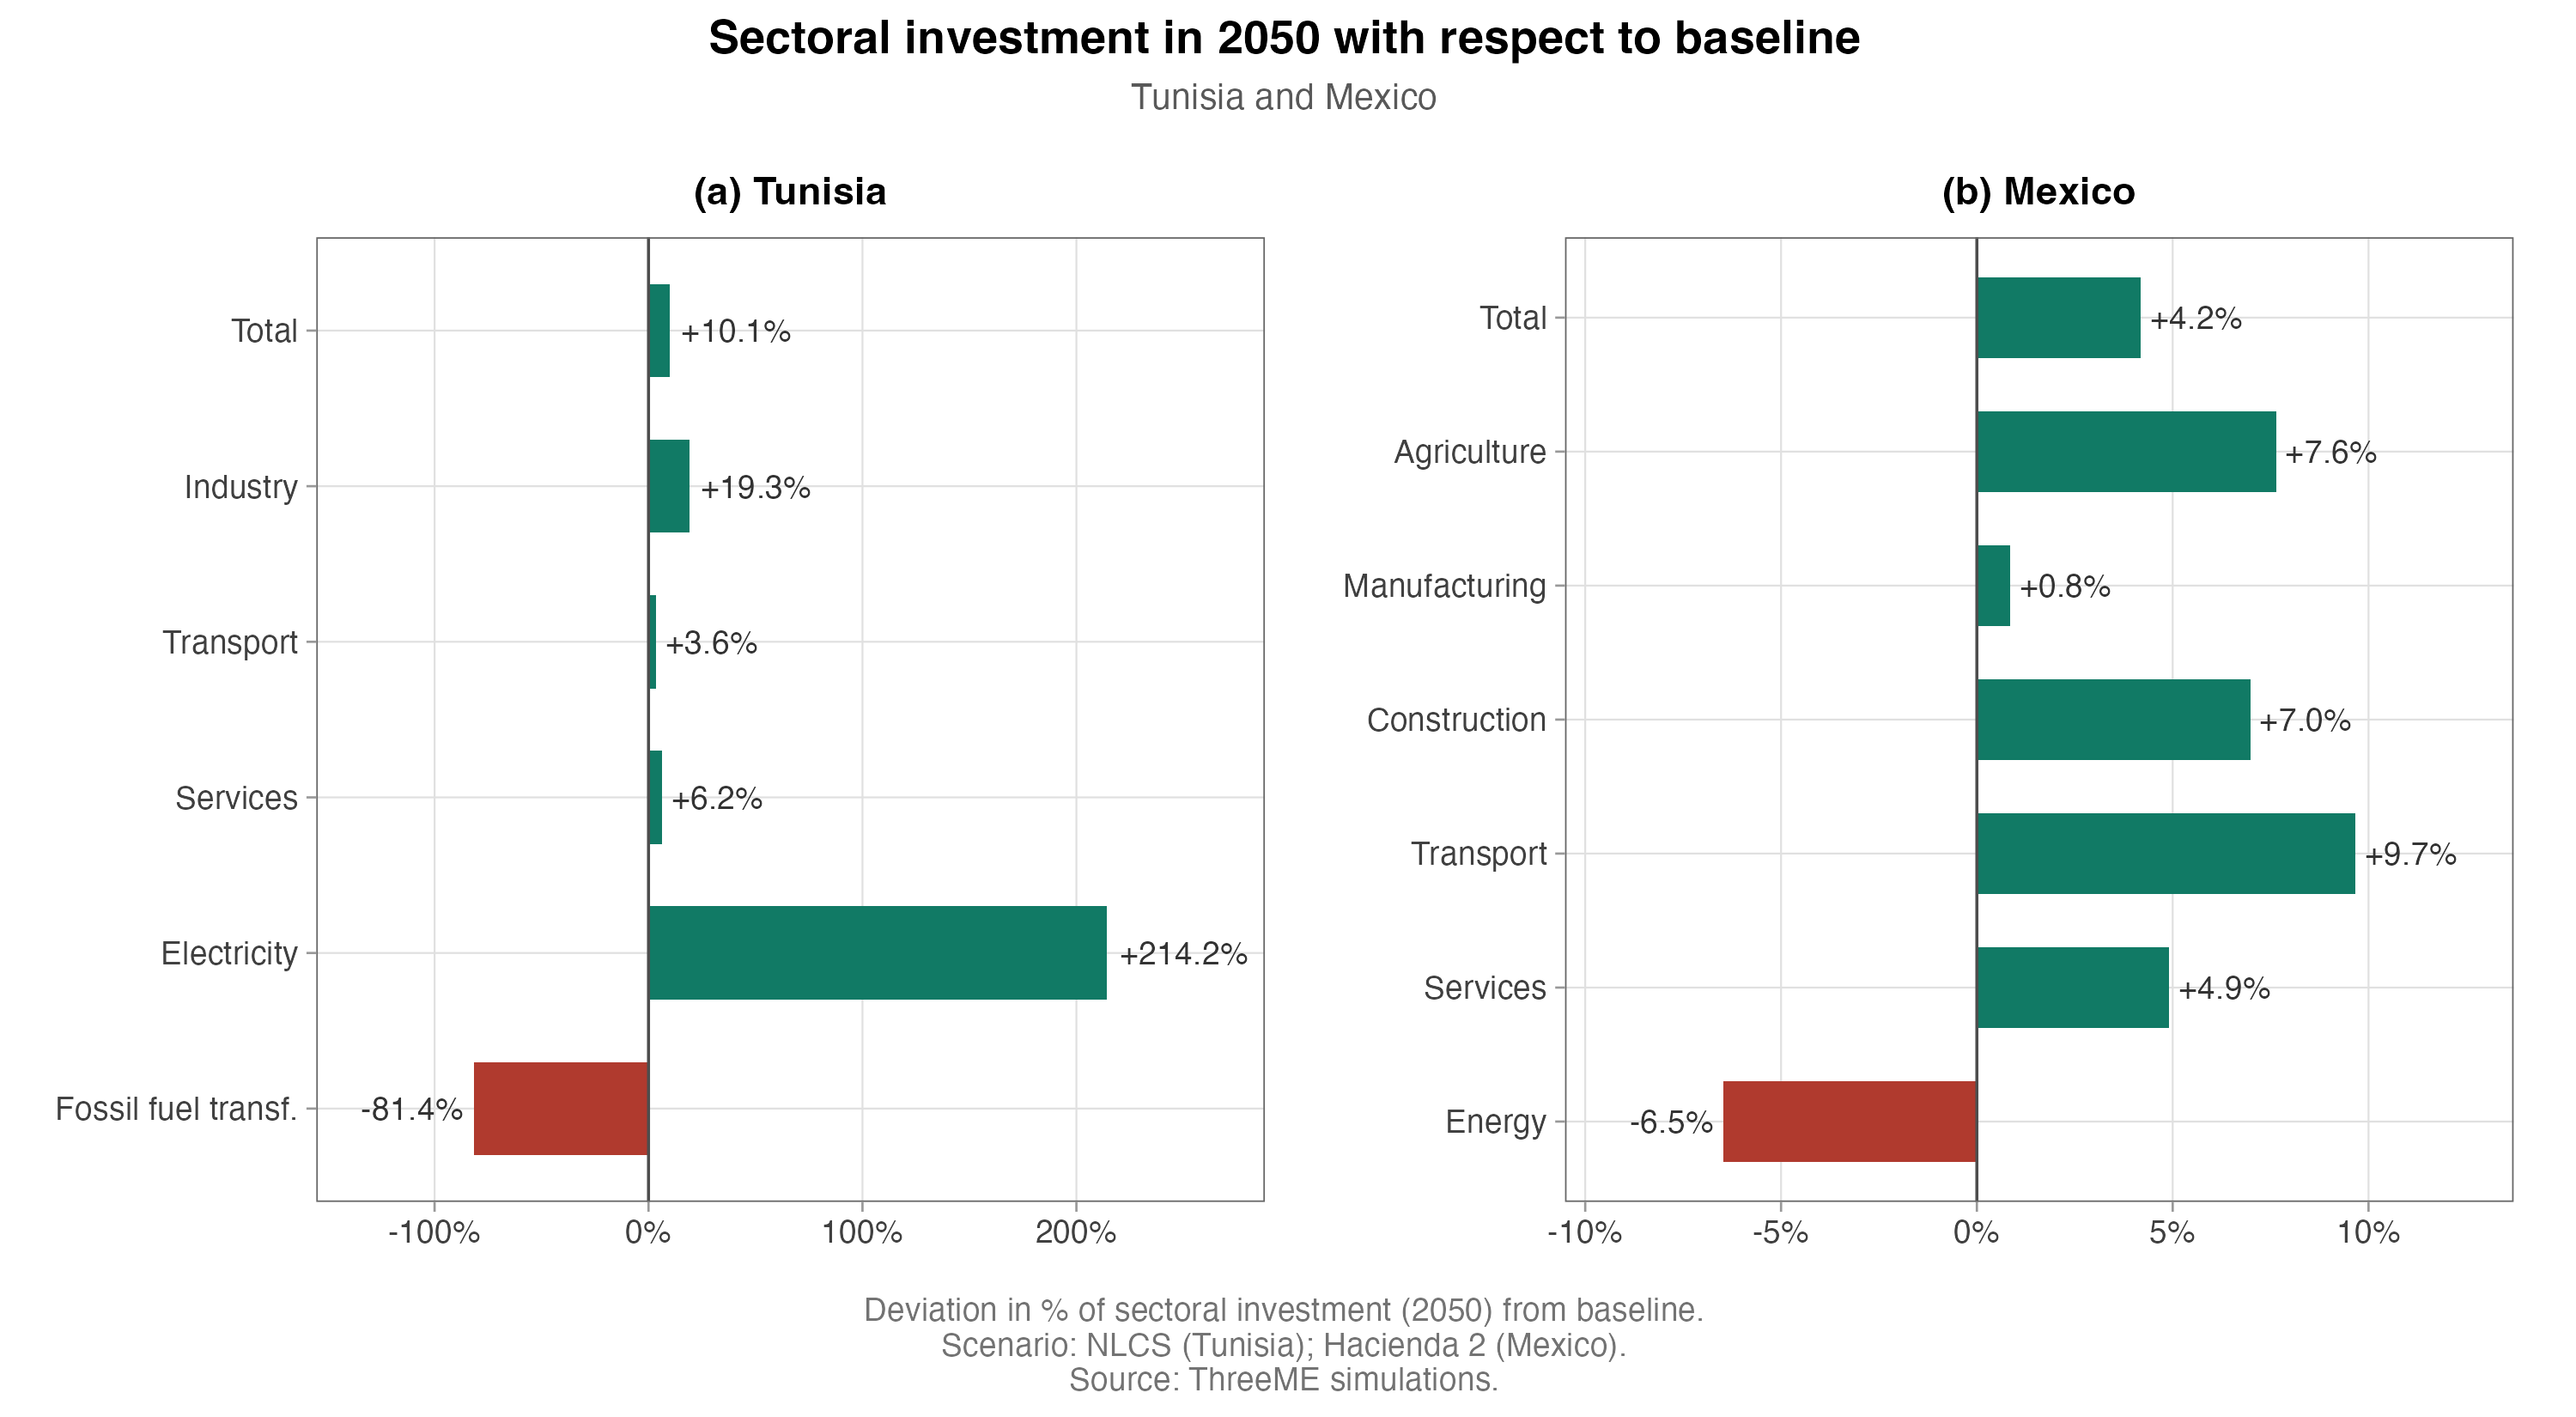
\includegraphics[width=0.95\textwidth]{fig10_investissement_sectoriel.png}
    \caption{Impact sur l'investissement par secteur en 2050 -- Tunisie (SNBC) et Mexique}
    \label{fig:invest_sectoral}
\end{figure}

L'analyse sectorielle de l'investissement (Figure~\ref{fig:invest_sectoral}) révèle des dynamiques contrastées entre les deux pays. La stratégie bas carbone induit une augmentation significative des investissements dans certains secteurs, notamment l'industrie et l'électricité. Étant donné qu'une très forte contrainte sur le renouvellement du mix électrique est imposée, on observe une augmentation significative des investissements dans le secteur électrique. En Tunisie, l'investissement dans ce secteur augmente de +66\,\% en 2030, +160\,\% en 2040 et +210\,\% en 2050 par rapport au scénario de référence. Un effet de substitution se produit alors : on observe simultanément une diminution importante des investissements dans les énergies fossiles.

\subsection{Consommation d'énergie et émissions par secteur}
\label{subsec:energie_emissions}

Les chocs induits par la levée des subventions aux énergies fossiles ainsi que l'introduction d'une taxe carbone génèrent une diminution de la consommation d'énergie des ménages et des secteurs productifs. Pour la Tunisie, la consommation d'énergie des ménages diminue de 8\,\% dès la première année par rapport au scénario de référence, et cet écart ne cesse de s'accentuer pour atteindre 36\,\% à l'horizon 2050.

\begin{figure}[H]
    \centering
    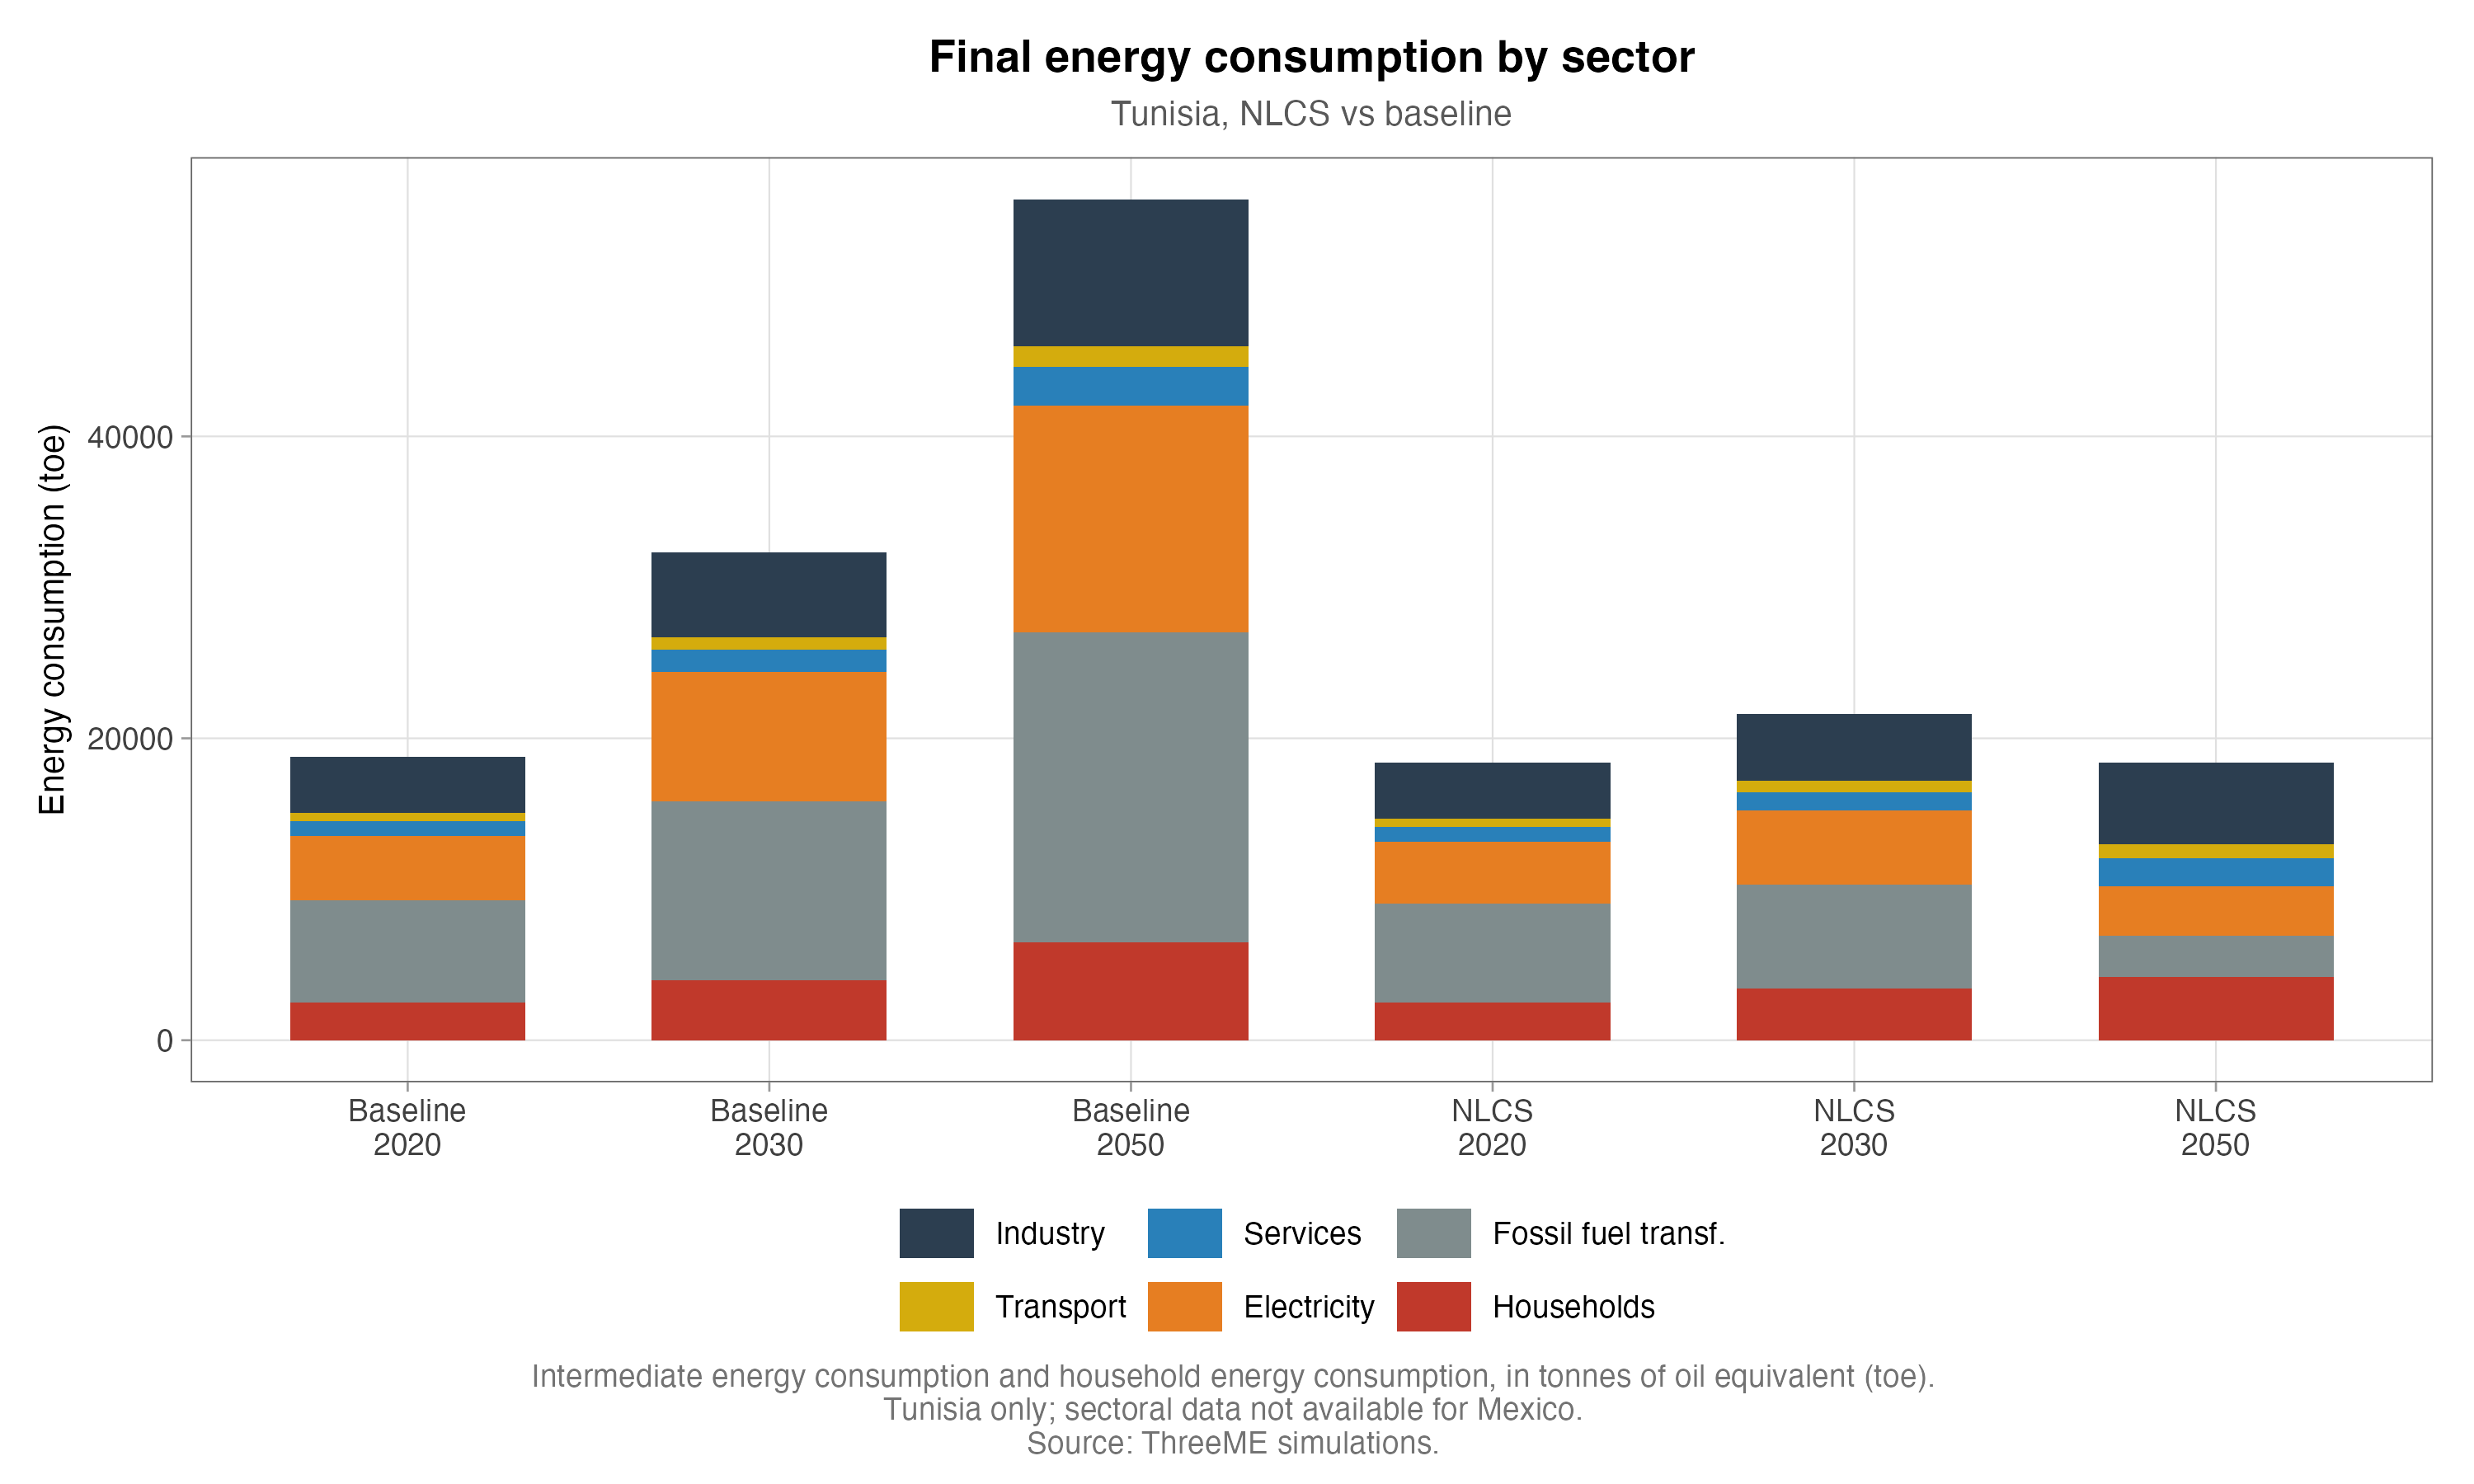
\includegraphics[width=0.95\textwidth]{fig11_energie_sectorielle.png}
    \caption{Consommation d'énergie finale par secteur -- Tunisie (scénario SNBC vs.\ référence)}
    \label{fig:energie_secteur}
\end{figure}

Aux vues de l'électrification massive des usages et de la pénétration significative des ENR dans le mix électrique, cette diminution de la consommation des ménages s'accompagne d'une diminution encore plus importante de leurs émissions de CO$_2$ (Figure~\ref{fig:co2_secteur}). Les émissions de CO$_2$ des ménages tunisiens baissent de 60\,\% en 2050, passant de 13\,MtCO$_2$ dans le scénario de référence à 5\,MtCO$_2$.

\begin{figure}[H]
    \centering
    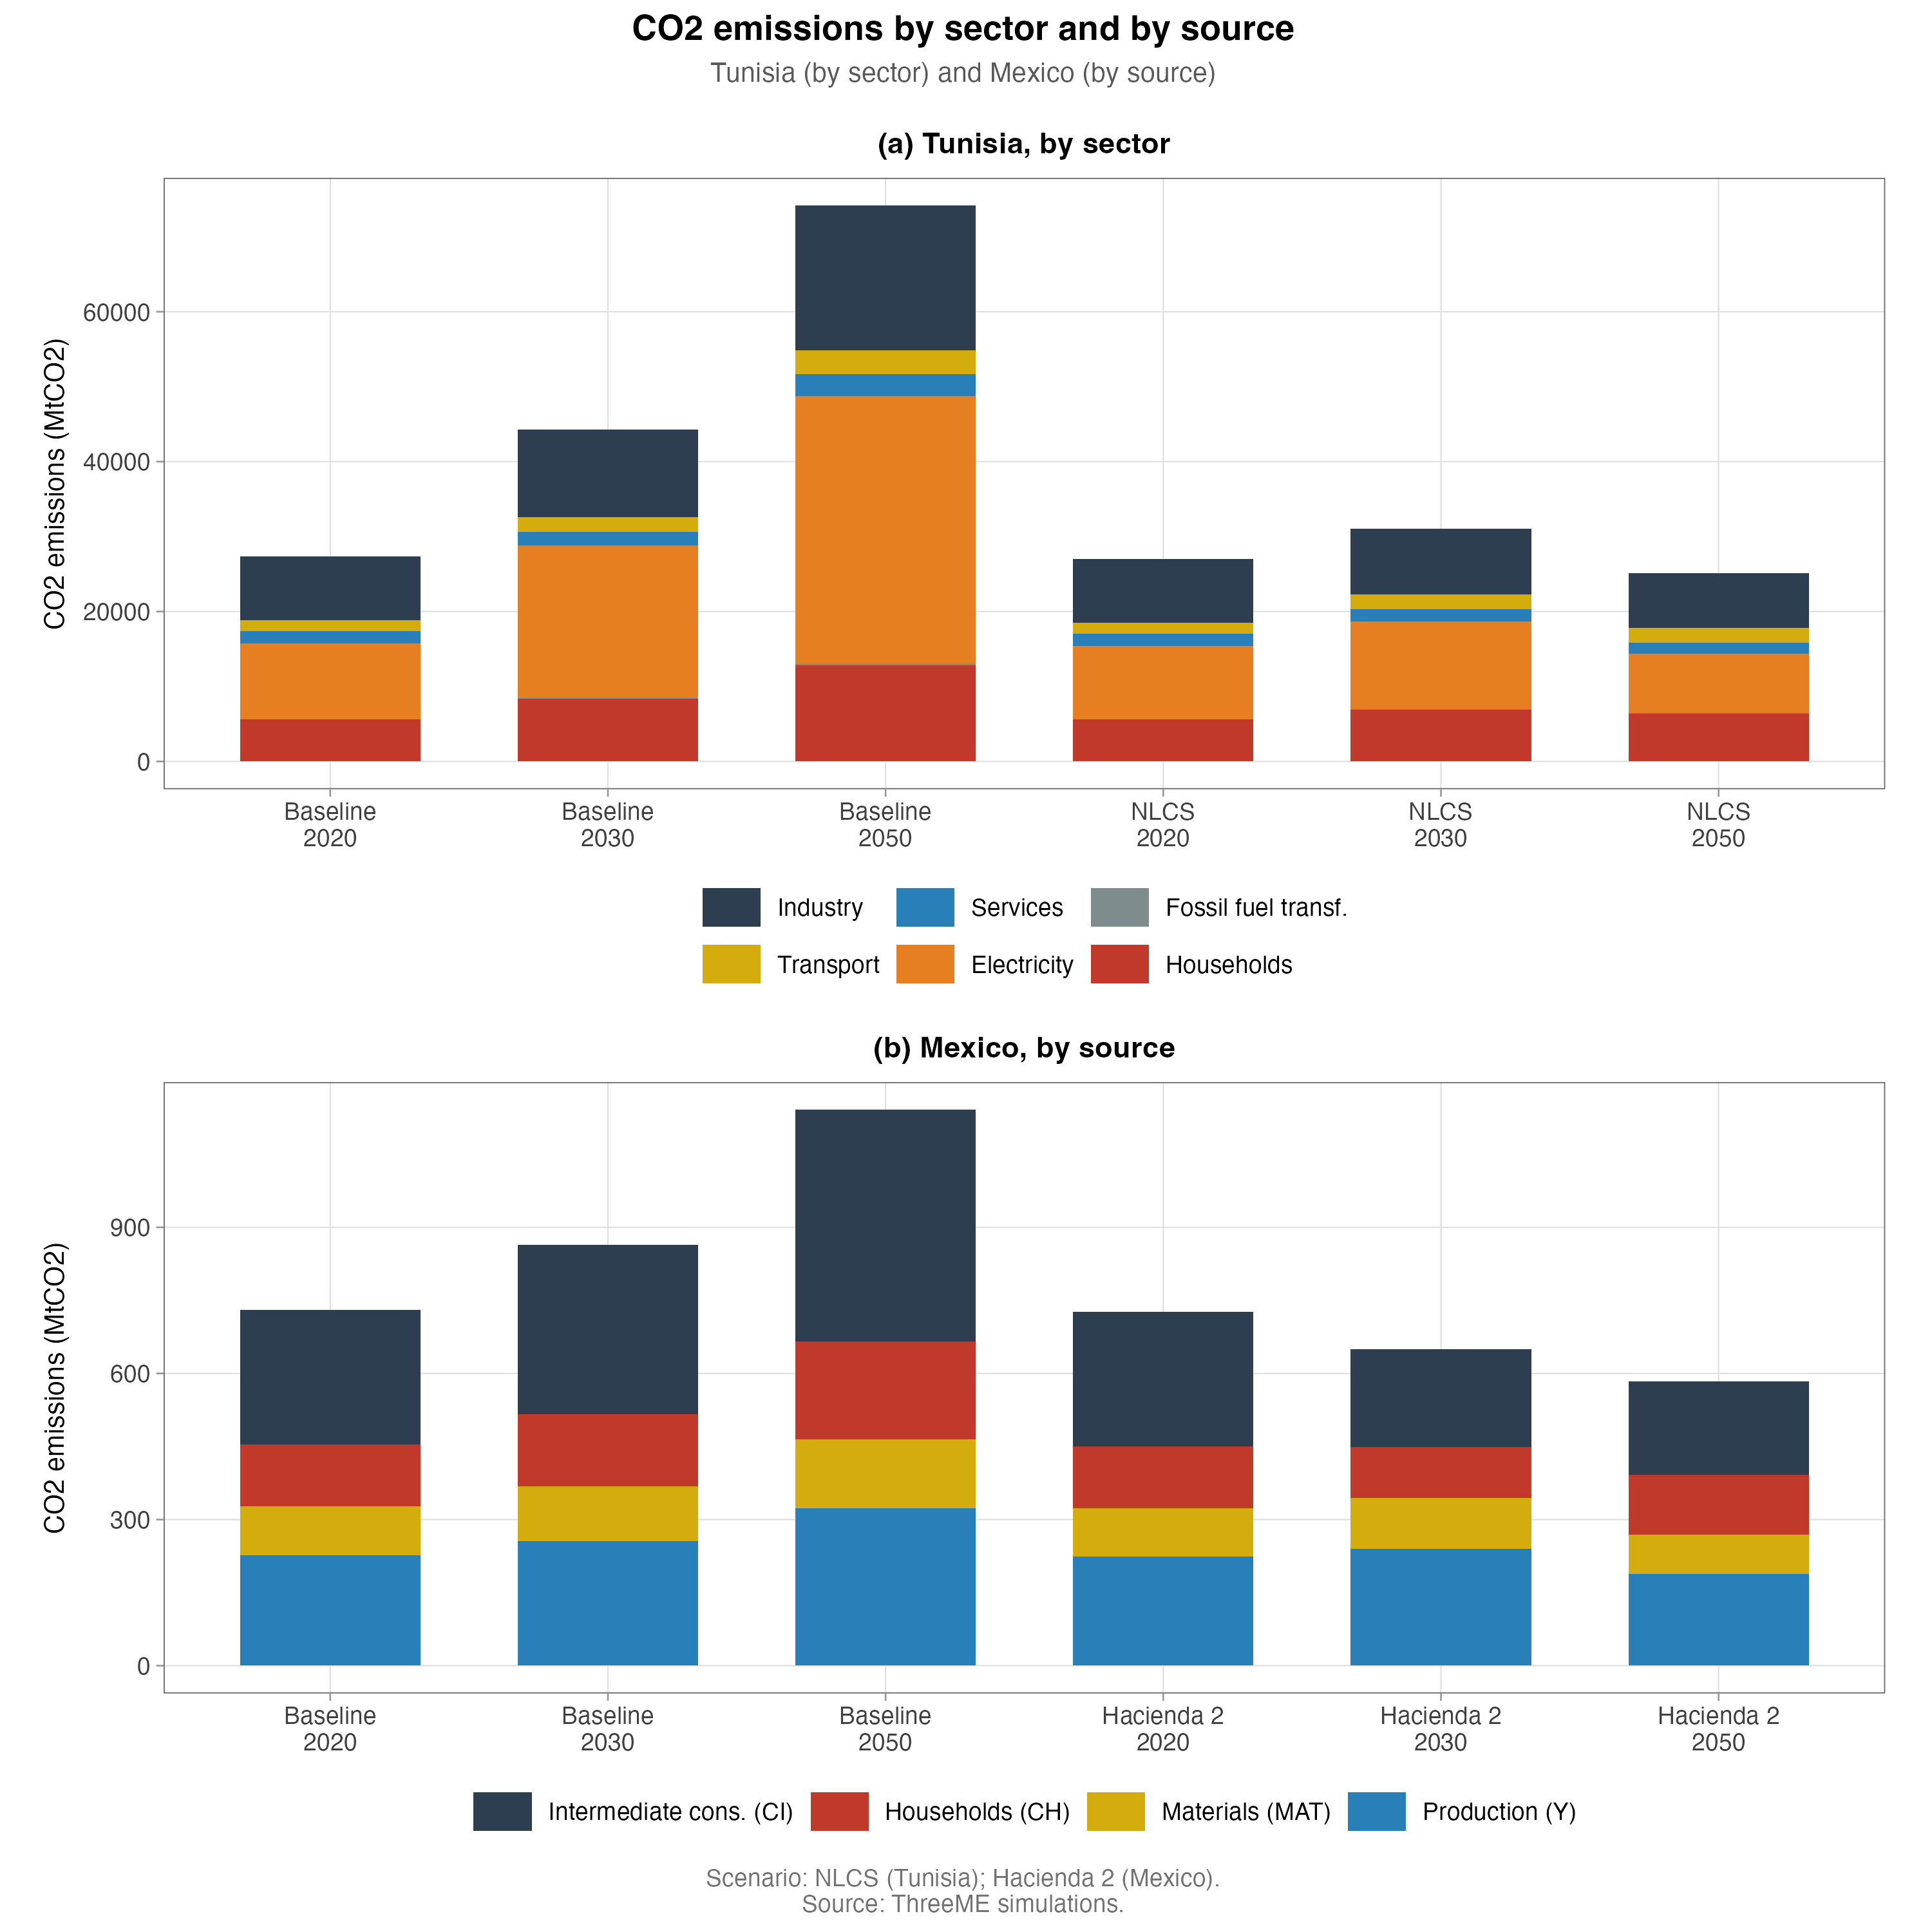
\includegraphics[width=0.95\textwidth]{fig12_co2_sectoriel.png}
    \caption{Émissions de CO$_2$ par secteur -- Tunisie (SNBC vs.\ référence) et Mexique (par source)}
    \label{fig:co2_secteur}
\end{figure}

On observe les mêmes phénomènes dans les secteurs productifs mais avec une intensité moins forte au début de la mise en place des politiques. En revanche, le phénomène de diminution de la consommation d'énergie est plus accentué en fin de période pour ces secteurs : là où les ménages diminuent leur consommation de 36\,\% en 2050, les secteurs productifs la diminuent de 69\,\%. De même pour les émissions, l'efficacité énergétique et la pénétration des ENR dans le mix électrique contribuent à une diminution significative : $-57$\,\% dans les services, $-65$\,\% dans l'industrie et $-85$\,\% dans l'électricité en 2050 par rapport au scénario de référence.

\subsection{Réallocation sectorielle de la valeur ajoutée}
\label{subsec:reallocation}

\begin{figure}[H]
    \centering
    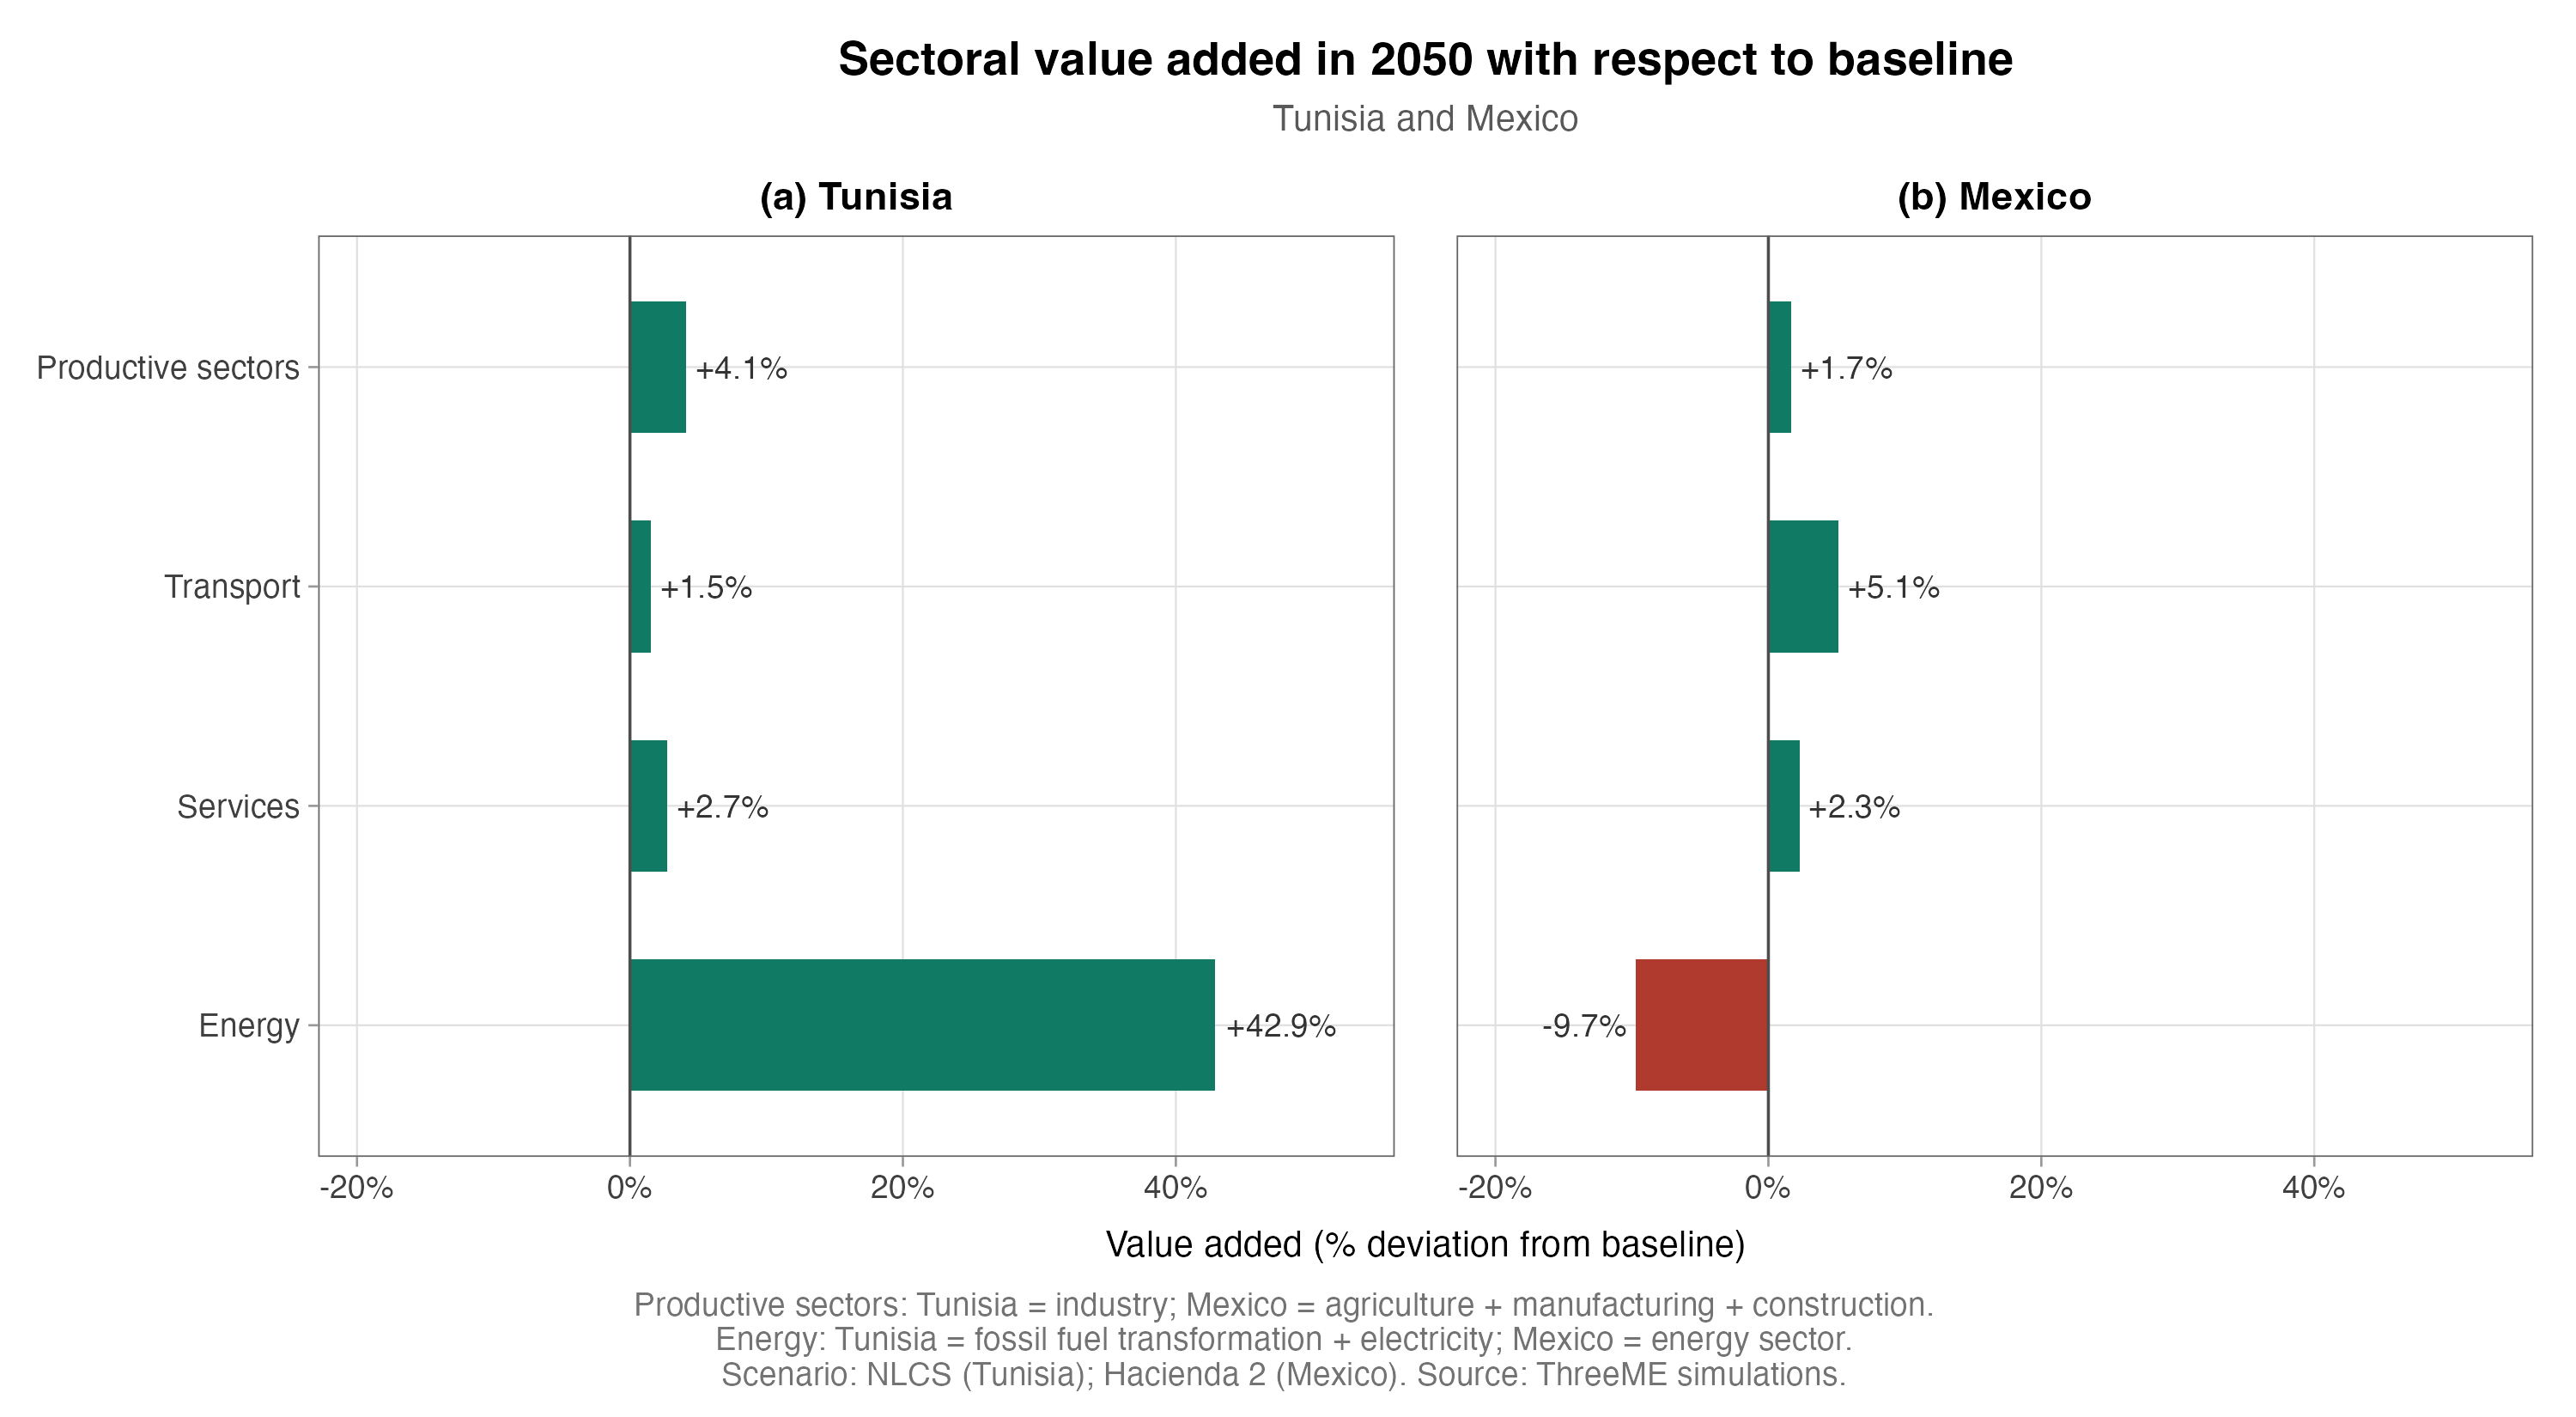
\includegraphics[width=0.95\textwidth]{fig06_va_sectorielle.png}
    \caption{Réallocation sectorielle de la valeur ajoutée -- Tunisie et Mexique}
    \label{fig:sectoral_va}
\end{figure}

Si les secteurs des services, transports et de l'industrie restent relativement stables et connaissent des évolutions comparables entre la Tunisie et le Mexique, le secteur de l'énergie subit des variations fortes et contraires dans les deux pays (Figure~\ref{fig:sectoral_va}).

D'un côté, le secteur de l'énergie est en recul de 7\,\% par rapport au scénario de référence pour le Mexique. L'instauration de la taxe carbone rend les exportations d'hydrocarbures fossiles moins compétitives : c'est la fin de la rente fossile dont bénéficiait le Mexique. Au contraire, la transition permet à la Tunisie de réduire sa dépendance extérieure à des hydrocarbures importés. Le développement des énergies renouvelables permet une forte croissance du secteur énergétique par la relocalisation de la production.

Un autre mécanisme entre en jeu : l'amélioration de la compétitivité-prix des secteurs exportateurs (industrie manufacturière et services), financée par la réduction des impôts de production grâce aux revenus de la taxe carbone.

\subsection{Effets sur le marché de l'emploi}
\label{subsec:emploi}

L'un des enseignements les plus marquants des simulations concerne les effets sur le marché du travail, qui se matérialisent progressivement dans le temps selon l'intensité et la combinaison des politiques mises en \oe{}uvre. En Tunisie, le scénario SNBC intégré entraîne une création nette de 51\,000 emplois dès 2030, qui s'amplifie régulièrement pour atteindre 194\,000 emplois supplémentaires en 2050. Ces résultats témoignent de la capacité de la transition à mobiliser de nouvelles compétences, à stimuler les investissements privés et publics, et à réorienter le tissu productif vers des secteurs plus intensifs en emploi.

\begin{figure}[H]
    \centering
    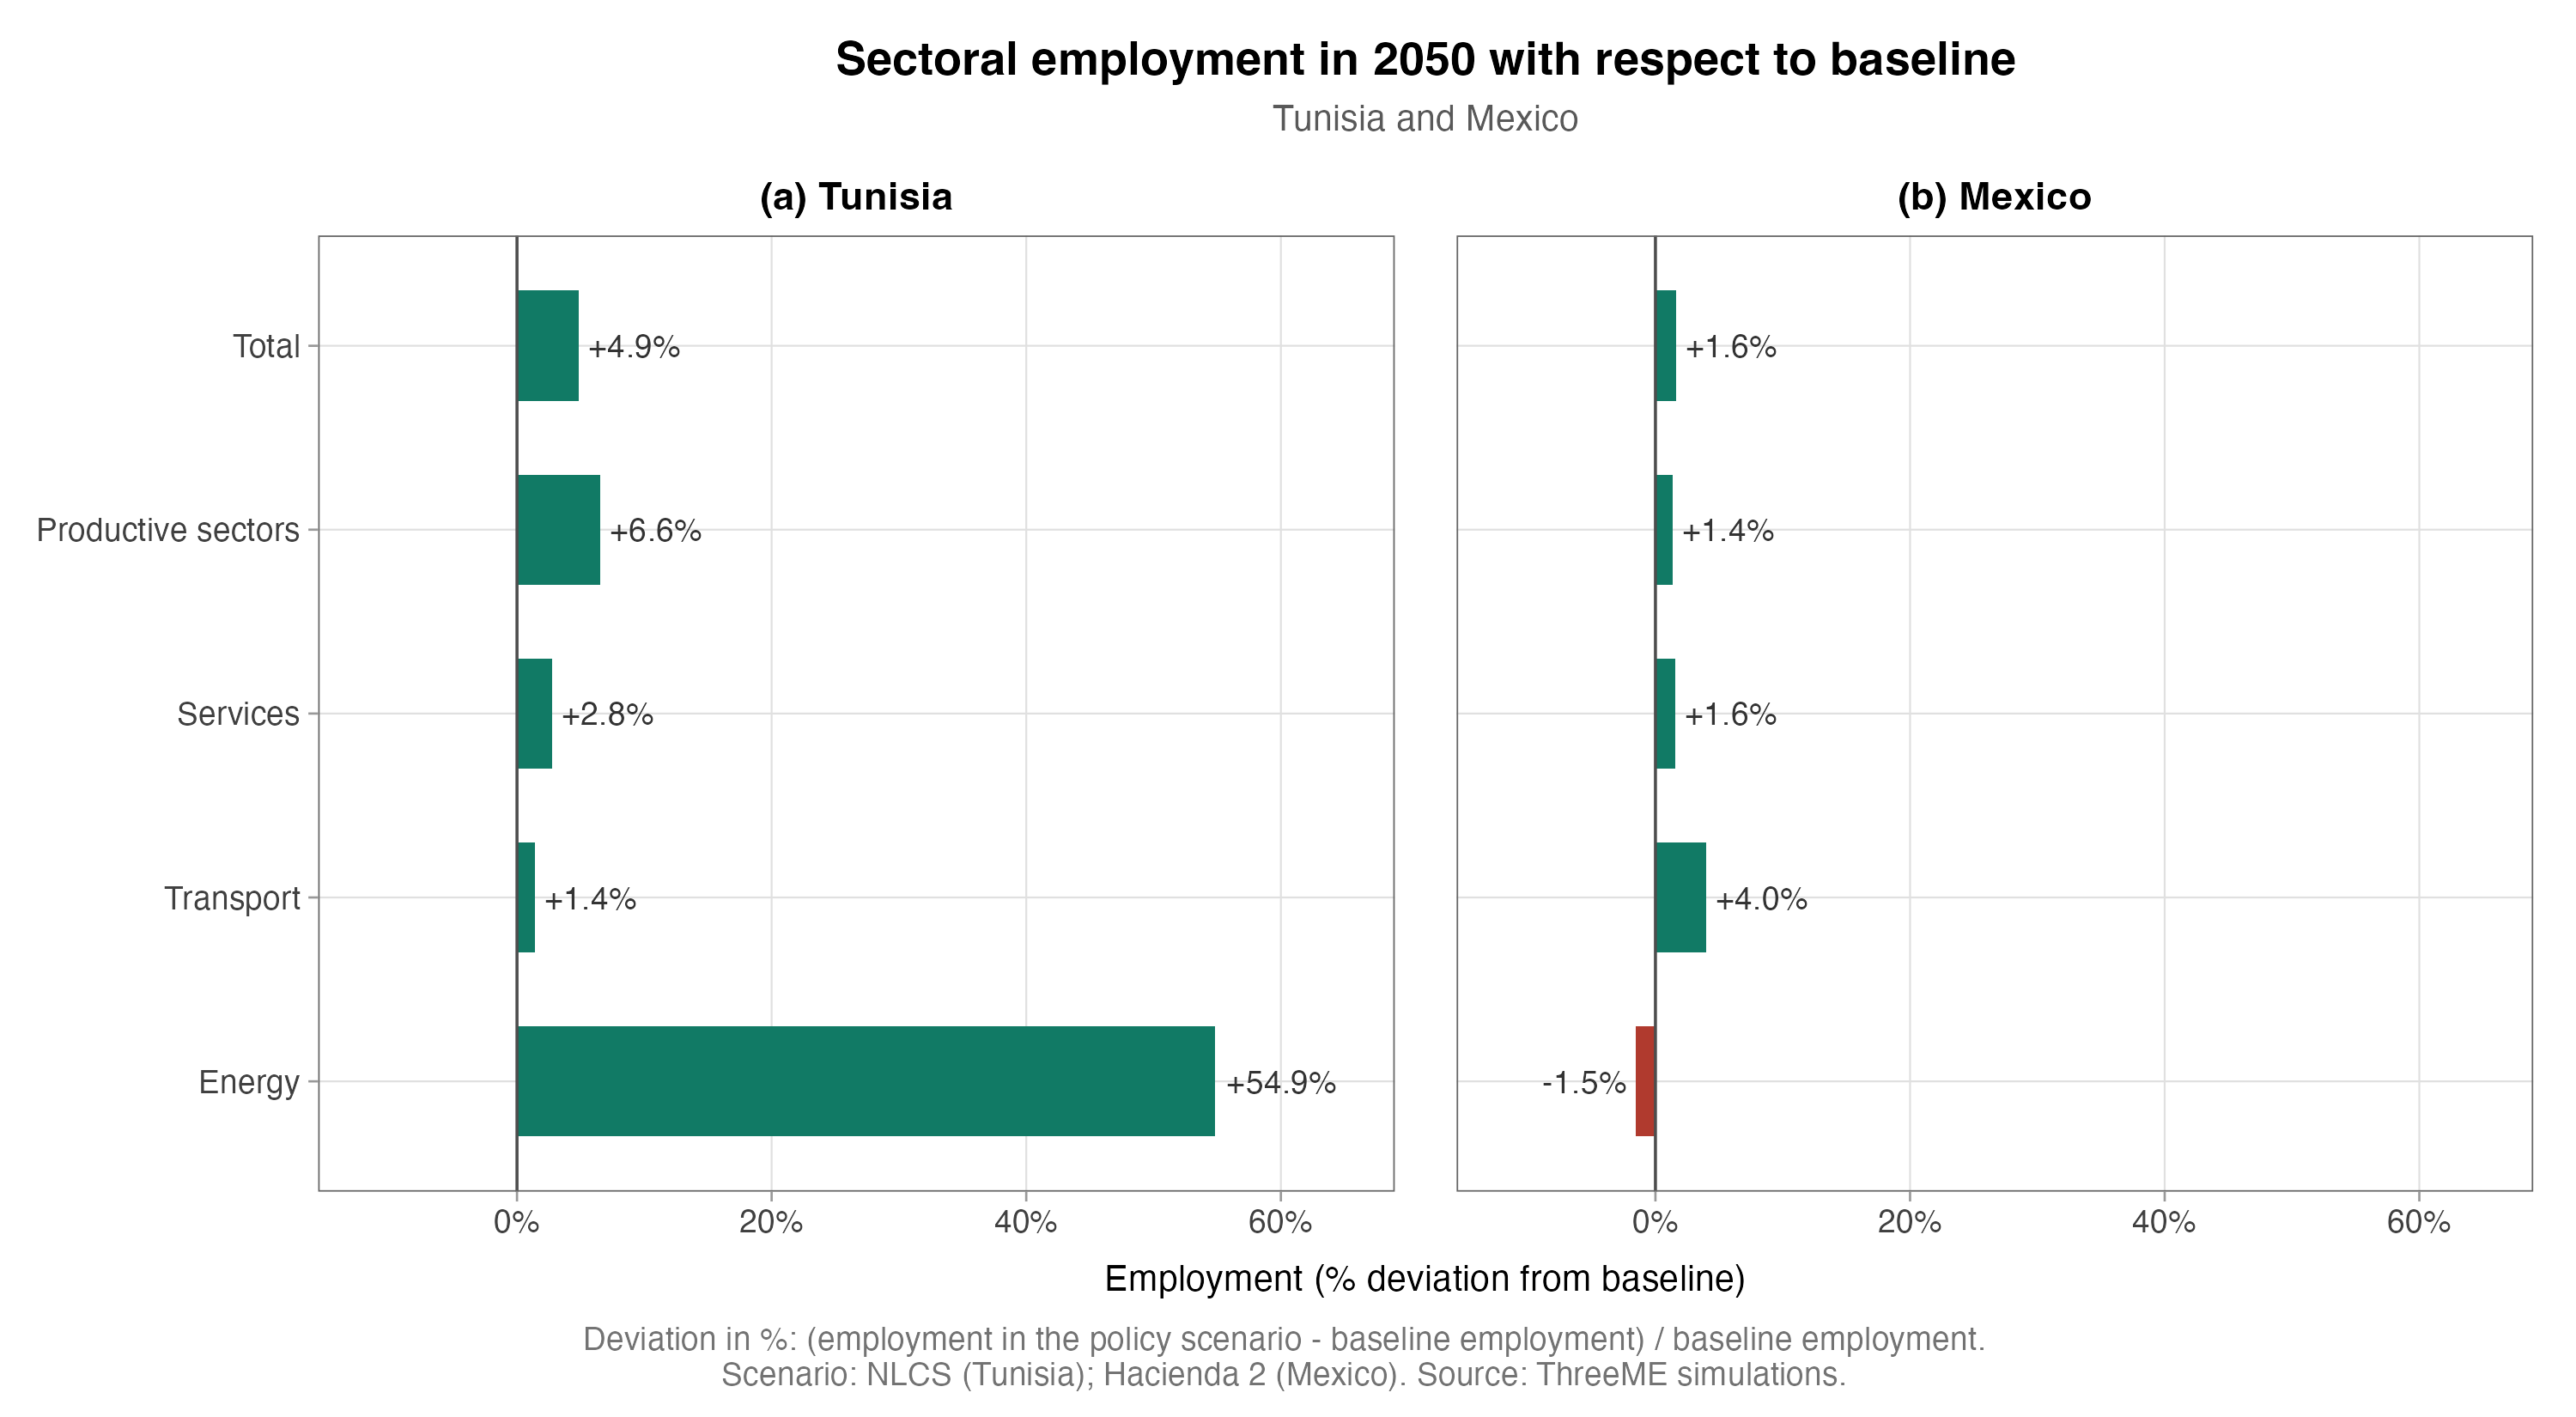
\includegraphics[width=0.95\textwidth]{fig07_emploi_sectoriel.png}
    \caption{Effets sectoriels sur l'emploi -- Mexique}
    \label{fig:employment_sectors}
\end{figure}

Pour le Mexique (Figure~\ref{fig:employment_sectors}), les créations d'emploi au niveau agrégé atteignent plus d'un million d'emplois en 2050, mais l'analyse sectorielle montre que l'emploi du secteur manufacturier décroche de près de 200\,000 emplois en 2050, mettant en évidence les effets de réallocation structurelle qui créent des gagnants et des perdants. L'enjeu pour le Mexique reste la reconversion entre l'exportation de pétrole brut et le développement de ses autres secteurs.

\subsection{Balance commerciale et insertion extérieure}
\label{subsec:balance_commerciale}

\begin{figure}[H]
    \centering
    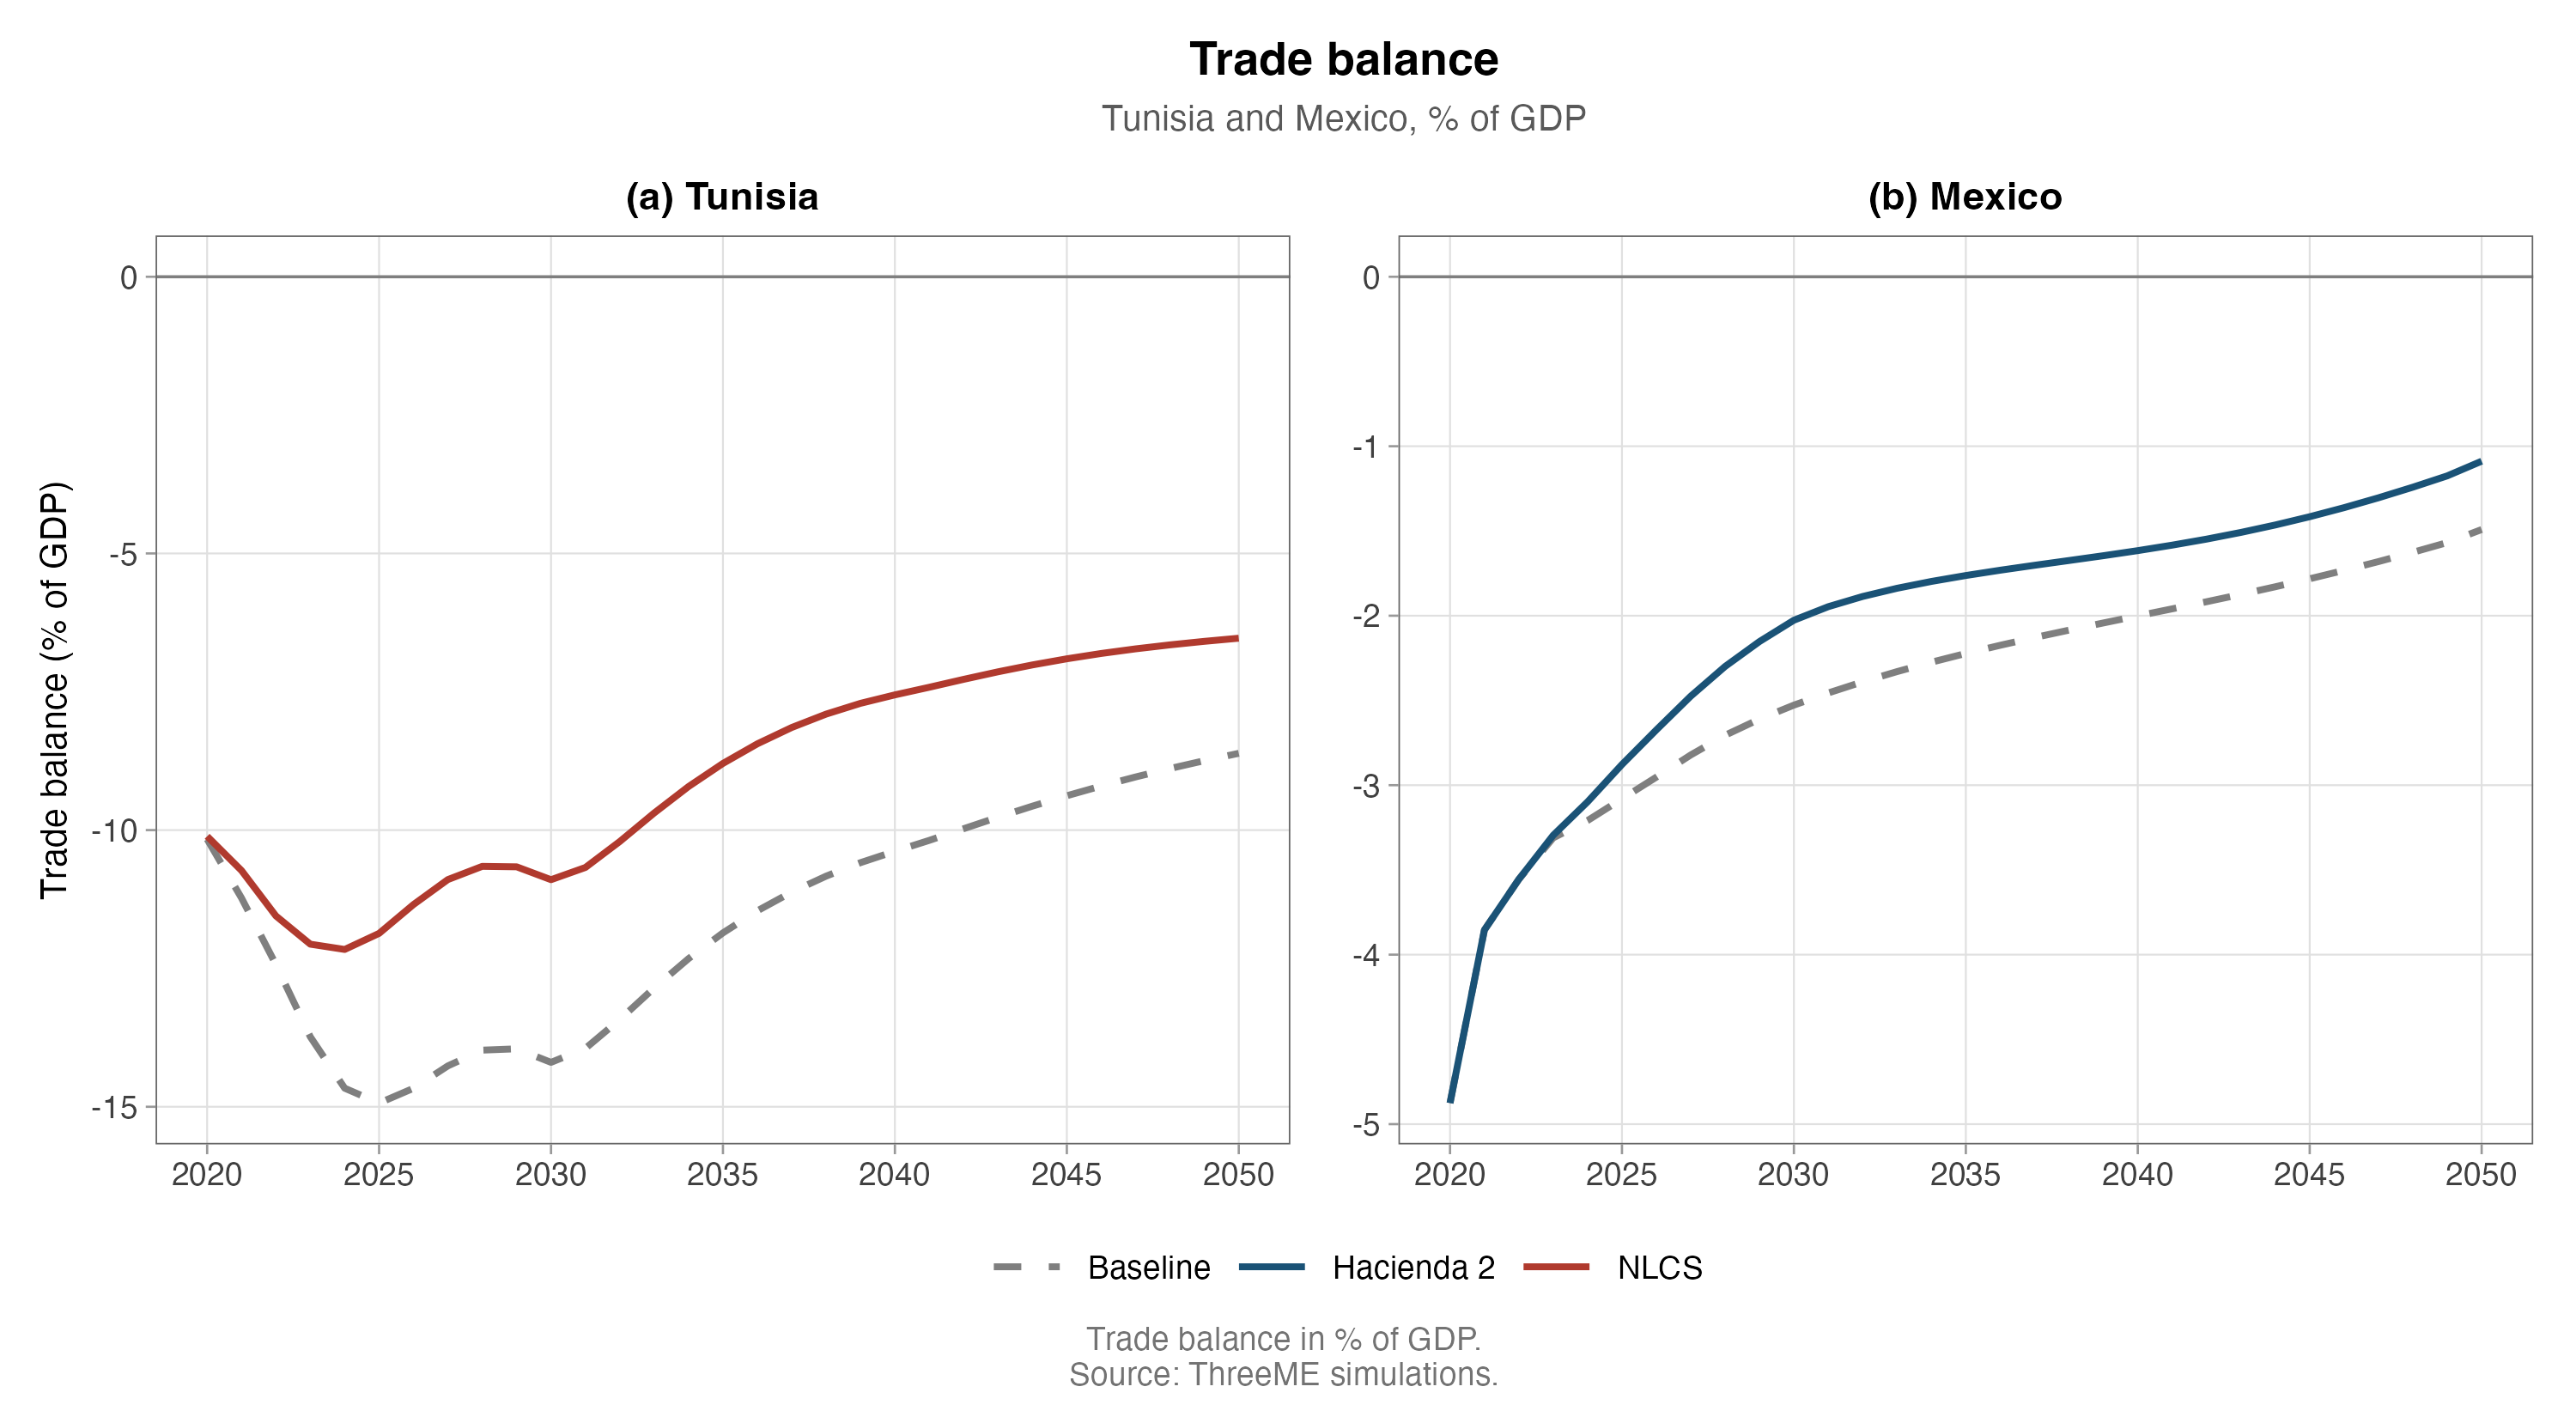
\includegraphics[width=0.95\textwidth]{fig13_balance_commerciale.png}
    \caption{Balance commerciale -- Tunisie et Mexique (écarts au scénario de référence)}
    \label{fig:trade_balance}
\end{figure}

La balance commerciale constitue un indicateur révélateur de l'asymétrie entre les deux pays (Figure~\ref{fig:trade_balance}). En Tunisie, la réduction progressive des importations de combustibles fossiles améliore mécaniquement le solde commercial, renforçant la souveraineté énergétique du pays. Toutefois, cette amélioration est partiellement contrebalancée par une hausse des importations de biens d'équipement nécessaires au déploiement des infrastructures renouvelables, en particulier lorsque les capacités industrielles locales ne sont pas encore pleinement développées. La dynamique économique endogène, soutenue par la consommation et l'investissement, génère également une demande additionnelle d'importations.

Au Mexique, l'effet sur la balance commerciale est plus contrasté. La baisse des exportations d'hydrocarbures pèse directement sur le solde commercial, tandis que le développement des secteurs renouvelables ne compense que partiellement cette perte, le Mexique devant également importer des technologies et biens d'équipement pour sa transition.

% ========================================
% 5. DISCUSSION
% ========================================
\section{Discussion : réalisme du découplage et limites}
\label{sec:discussion}

Les résultats présentés suggèrent que pour la Tunisie comme pour le Mexique, un découplage s'opère entre croissance du produit intérieur brut et croissance des émissions. Cette observation dépend toutefois d'hypothèses de modélisation dont il convient de discuter la robustesse.

\textbf{Les élasticités de substitution capital-énergie} déterminent la manière dont les entreprises remplacent l'énergie fossile par du capital productif en réponse au signal-prix. Plus l'élasticité est grande, plus le découplage s'opère facilement, or ce paramètre est débattu empiriquement (Landa et Reynès, 2025). \textbf{La pénétration des ENR} est un paramètre du scénario imposé de manière exogène (80\,\% pour la Tunisie et 50\,\% pour le Mexique). Si le déploiement s'avère plus difficile ou coûteux que prévu, un découplage différent serait observé. \textbf{Le recyclage fiscal} augmente le numérateur du ratio croissance du PIB / croissance des émissions de manière mécanique ; la décarbonation effective de l'appareil productif procède d'un mécanisme séparé de l'effet macroéconomique.

Par ailleurs, ces hypothèses se confrontent à des réalités empiriques contradictoires. Haberl et al. (2020) montrent que les exemples de découplage absolu à long terme restent rares. Même si certaines économies post-industrielles ont réalisé ce découplage, il ne serait pas suffisamment rapide pour atteindre les objectifs de l'accord de Paris (Hickel et Kallis, 2020). Le mécanisme de découplage peut également être surestimé par le périmètre territorial des émissions, qui ne capture pas les fuites de carbone : les biens carbonés pourraient être importés par la Tunisie plutôt que produits sur place.

Certains coûts liés à la transition ne sont pas modélisés dans ThreeME : la part informelle de l'économie tunisienne, le lien étroit entre PEMEX et les finances publiques au Mexique, et la formation nécessaire à la restructuration du marché de l'emploi. De plus, les modèles d'équilibre général tels que ThreeME ne capturent qu'une partie des effets rebond, essentiellement le rebond direct des ménages via les prix et le revenu réel, en laissant de côté de nombreux mécanismes macroéconomiques à l'échelle de l'économie (Brockway et al., 2021).

Enfin, la comparabilité des résultats entre les deux pays est limitée par le fait que les deux versions du modèle ont été développées et calibrées indépendamment. Les différences de structure sectorielle, de nombre de secteurs, de calibration des paramètres comportementaux et d'hypothèses sur le scénario de référence invitent à une lecture comparative centrée sur les mécanismes qualitatifs plutôt que sur les magnitudes absolues.

Les résultats démontrant un découplage sont donc fortement conditionnés. Les enseignements à tirer ne sont pas les précisions quantitatives apportées par les simulations, mais l'illustration des mécanismes à l'\oe{}uvre dans les asymétries entre importateurs et exportateurs lors de la transition.

% ========================================
% 6. CONCLUSION
% ========================================
\section{Conclusion}
\label{sec:conclusion}

Cet article propose une évaluation des effets macroéconomiques de la mise en \oe{}uvre de stratégies nationales bas carbone dans deux économies en développement aux profils énergétiques contrastés : la Tunisie, importatrice nette d'hydrocarbures, et le Mexique, exportateur net. À l'aide du modèle d'équilibre général calculable néo-keynésien ThreeME, nous simulons des scénarios de transition ambitieux à l'horizon 2050.

En plus du dividende environnemental obtenu par construction, nos simulations montrent que les politiques de transition peuvent conduire à un dividende économique : augmentation de l'investissement, créations d'emplois dans les industries vertes nettement supérieures aux destructions dans les secteurs intensifs en énergie fossile. Malgré la hausse des prix de l'énergie, la demande augmente et le PIB est supérieur au scénario de référence. Pour la Tunisie, la transition induit un gain de PIB de l'ordre de +5\,\% et un gain d'emploi significatif en 2050. Pour le Mexique, le gain est positif mais plus modéré, reflétant le coût de la restructuration du secteur extractif.

La comparaison entre la Tunisie et le Mexique met en évidence le caractère asymétrique du choc de transition. Pour un pays importateur net d'énergie, la réduction de la facture énergétique extérieure et la montée de l'investissement domestique transforment la transition en levier de relance et d'amélioration de la balance commerciale. À l'inverse, pour un pays exportateur d'hydrocarbures, la transition implique un processus plus coûteux de réallocation sectorielle, marqué par le déclin d'un secteur historiquement central et par des besoins accrus d'accompagnement productif et social. Les résultats soulignent également l'importance de la dynamique temporelle : les effets sont d'abord dominés par l'investissement, avant que les réallocations structurelles ne deviennent prépondérantes à mesure que le prix du carbone augmente.

Le recyclage intégral des recettes fiscales --- sous forme de transferts aux ménages et de soutien à l'investissement productif des entreprises --- apparaît comme une condition nécessaire à l'obtention du double dividende. En l'absence de recyclage, les scénarios tunisiens montrent une contraction du PIB par rapport à la baseline, confirmant que le mode de redistribution des recettes est aussi déterminant que le niveau de la taxe elle-même.

Comme discuté dans la section~\ref{sec:discussion}, le découplage observé dans les simulations repose sur un ensemble d'hypothèses structurantes dont la réalisation n'est pas garantie. Le modèle ne capture ni les fuites de carbone, ni l'hétérogénéité des ménages, ni les coûts de reconversion professionnelle, ce qui invite à interpréter les résultats quantitatifs avec prudence.

Ces limites n'enlèvent pas la portée qualitative des enseignements principaux. Au-delà des cas tunisien et mexicain, cette étude suggère que la transition bas carbone, dans les pays en développement, doit être envisagée comme une stratégie de transformation économique de long terme. Elle ne constitue pas uniquement une contrainte climatique, mais aussi un levier potentiel de réorientation du modèle de croissance, à condition d'être accompagnée de politiques budgétaires, industrielles et sociales cohérentes. Les travaux futurs pourraient approfondir l'analyse en intégrant une désagrégation plus fine des ménages, une représentation explicite des politiques de formation et de reconversion, ainsi qu'une modélisation des interactions commerciales multilatérales permettant de traiter la question des fuites de carbone.

% ========================================
% BIBLIOGRAPHIE
% ========================================
\newpage
\section*{Références}
\addcontentsline{toc}{section}{Références}

\begin{enumerate}[label={[\arabic*]}, leftmargin=*]

\item ANME (2020). Plan Solaire Tunisien : études sur le potentiel des énergies renouvelables et de l'efficacité énergétique. Agence Nationale pour la Maîtrise de l'Énergie.

\item Aubert, D., \& Chiroleu-Assouline, M. (2019). Environmental tax reform and income distribution with imperfect heterogeneous labour markets. \textit{European Economic Review}, 116, 60--82.

\item Babonneau, F., Badran, A., Haurie, A., et al. (2023). GCC countries strategic options in a global transition to zero-net emissions. \textit{Environmental Modeling \& Assessment}, 28, 709--733.

\item Banque Mondiale (2023a). Tunisia Economic Monitor. Washington, DC.

\item Banque Mondiale (2023b). Country Climate and Development Report -- Tunisia.

\item Banque Mondiale (2024). World Development Indicators -- Tunisia.

\item Belhadj, A., Dakhlaoui, A., \& Gouider, R. (2022). Assessing macroeconomic, distributive, and environmental impacts of energy subsidy removal in Tunisia with input-output modeling. In \textit{Key Challenges and Policy Reforms in the MENA Region}, Springer, pp.~65--84.

\item Bento, A.~M., \& Jacobsen, M.~R. (2007). Ricardian rents, environmental policy and the `double-dividend' hypothesis. \textit{Journal of Environmental Economics and Management}, 53(1), 17--31.

\item Böhringer, C., Garcia-Muros, X., \& Gonzalez-Eguino, M. (2019). Greener and fairer: a progressive environmental tax reform for Spain. \textit{Economics of Energy \& Environmental Policy}, 8(2).

\item Böhringer, C., Rutherford, T.~F., \& Schneider, J. (2021). The incidence of CO$_2$ emissions pricing under alternative international market responses. \textit{Energy Economics}, 101, 105404.

\item Brockway, P.~E., et al. (2021). Energy efficiency and economy-wide rebound effects: A review of the evidence and its implications. \textit{Renewable and Sustainable Energy Reviews}, 141, 110781.

\item Bulavskaya, T., \& Reynès, F. (2018). Job creation and economic impact of renewable energy in the Netherlands. \textit{Renewable Energy}, 119, 528--538.

\item Callonnec, G., Landa, G., Malliet, P., Reynès, F., Tamsamani, Y. (2013). A full description of the ThreeME model. \textit{Document de travail OFCE}.

\item Callonnec, G., Landa, G., Malliet, P., Saussay, A., \& Reynès, F. (2016). Les propriétés dynamiques et de long terme du modèle ThreeME : un cahier de variantes. \textit{Revue de l'OFCE}, 149.

\item Callonnec, G., Gouëdard, H., Hamdi-Cherif, M., Landa, G., Malliet, P., Reynès, F., \& Saussay, A. (2025). Macroeconomic effects of achieving carbon neutrality in France. \textit{Energy and Climate Change}, 6, 100131.

\item Dridi, M. (2024). Tunisia: economic challenges and reform prospects. Working paper.

\item Elbargathi, K., \& Al-Assaf, G. (2019). The impact of political instability on the economic growth: an empirical analysis for the case of selected Arab countries. \textit{International Journal of Business and Economics Research}, 8(6), 353--360.

\item Fragkos, P., Fragkiadakis, K., \& Paroussos, L. (2021). Reducing the decarbonisation cost burden for EU energy-intensive industries. \textit{Energies}, 14(1), 236.

\item GIEC (2018). Réchauffement planétaire de 1,5\,$^{\circ}$C. Résumé à l'intention des décideurs. GIEC, Genève, Suisse.

\item Goulder, L.~H. (2013). Climate change policy's interactions with the tax system. \textit{Energy Economics}, 40(Suppl. 1), S3--S11.

\item Haberl, H., et al. (2020). A systematic review of the evidence on decoupling of GDP, resource use and GHG emissions. \textit{Environmental Research Letters}, 15(6), 065003.

\item Hamdi-Cherif, M., Reynès, F., Landa, G., \& Wang, J. (2025). Effets macroéconomiques et environnementaux de la SNBC en Tunisie -- Une analyse à court et long terme. \textit{Revue de l'OFCE}.

\item Hickel, J., \& Kallis, G. (2020). Is green growth possible? \textit{New Political Economy}, 25(4), 469--486.

\item IEA (2021). Net Zero by 2050: A Roadmap for the Global Energy Sector. International Energy Agency.

\item IPCC (2022). Climate Change 2022: Mitigation of Climate Change. Sixth Assessment Report.

\item Jacques, P., Augier, S., Barbosa, S., Yilmaz, S.~D., Jeanmart, H., \& Godin, A. (2025). Coupling a stock-flow consistent macroeconomic model with an energy system optimisation model to study the impacts of the energy transition in Colombia. \textit{SSRN Working Paper}, No.~5650377.

\item Jebali, E., et al. (2017). Energy consumption and economic growth in Tunisia. \textit{Journal of Policy Modeling}.

\item Kahn, J.~R., \& Farmer, A. (1999). The double dividend, second-best worlds, and real-world environmental policy. \textit{Ecological Economics}, 30, 433--439.

\item Karanfil, F., \& Omgba, L.~D. (2023). The energy transition and export diversification in oil-dependent countries: the role of structural factors. \textit{Ecological Economics}, 204, 107681.

\item Khouaja, A. (2020). Renewable energy potential in Tunisia: assessment and perspectives. Working paper.

\item Landa, G., Reynès, F., Islas, I., Bellocq, F.-X., \& Grazi, F. (2016). Towards a low carbon growth in Mexico: is a double dividend possible? A dynamic general equilibrium assessment. \textit{Energy Policy}, 96, 314--327.

\item Landa, G., \& Reynès, F. (2025). Les bienfaits économiques de l'action pour le climat : une illustration. \textit{Policy Brief OFCE}.

\item Landis, F., Fredriksson, G., \& Rausch, S. (2021). Between- and within-country distributional impacts from harmonizing carbon prices in the EU. \textit{Energy Economics}, 103, 105585.

\item Lepault, C., \& Lecocq, F. (2021). Mapping forward-looking mitigation studies at country level. \textit{Environmental Research Letters}, 16(8), 083001.

\item Lutz, C., Becker, L., \& Kemmler, A. (2021). Socioeconomic effects of ambitious climate mitigation policies in Germany. \textit{Sustainability}, 13(11), 6247.

\item Magacho, G., Espagne, E., Godin, A., Mantes, A., \& Yilmaz, D. (2023). Macroeconomic exposure of developing economies to low-carbon transition. \textit{World Development}, 167, 106231.

\item Malliet, P., Nazhiri, I., \& Reynès, F. (2016). Assessing low carbon and resilient growth in Indonesia: an application of the ThreeME model.

\item Maxim, M., Zander, K., \& Patuelli, R. (2019). Green tax reform and employment double dividend in European and non-European countries: a meta-regression assessment. \textit{International Journal of Energy Economics and Policy}, 9(4), 342--355.

\item Mraihi, R., \& Ben Salem, A. (2019). Energy consumption and economic growth in Tunisia. Working paper.

\item O'Ryan, R., Nasirov, S., \& Osorio, H. (2023). Assessment of the potential impacts of a carbon tax in Chile using dynamic CGE model. \textit{Journal of Cleaner Production}, 403, 136694.

\item Pearce, D.~W. (1991). The role of carbon taxes in adjusting to global warming. \textit{The Economic Journal}, 101(407), 938--948.

\item PNUD (2021). Analyses sectorielles sur la réduction des émissions et l'adaptation climatique en Tunisie.

\item Soummane, S., Ghersi, F., \& Lefèvre, J. (2019). Macroeconomic pathways of the Saudi economy: the challenge of global mitigation action versus the opportunity of national energy reforms. \textit{Energy Policy}, 130, 263--282.

\item Sovacool, B.~K., et al. (2015). Integrating social science in energy research. \textit{Energy Research \& Social Science}, 6, 95--99.

\item UNFCCC (2015). Accord de Paris. Convention-Cadre des Nations Unies sur les Changements Climatiques.

\item Zaghdoud, O. (2025). Environmental fiscal policies and the double dividend hypothesis: a dynamic CGE-OLG analysis in Tunisia. \textit{Economics}.

\end{enumerate}

\end{document}
